\graphicspath{{Dissertation/images/chapt2/}}

\chapter{Наземно-космический интерферометр <<РадиоАстрон>>} \label{chapt2}

% TODO: ужасный язык -- переписать
Автоматический космический аппарат <<Спектр-Р>> предназначен для установки на нем космического
радиотелескопа, используемого в качестве орбитального плеча наземно-космического
радиоинтерферометра со сверхдлинными базами (РСДБ). В его состав входят базовый служебный модуль
<<Навигатор>> (головная организация~"--- НПО им. С.А. Лавочкина) [21] и научный комплекс, состоящий
из научной аппаратуры космического радиотелескопа международного проекта <<РадиоАстрон>> (головная
организация~"--- АКЦ ФИАН) и параболической антенны диаметром 10 м (совместная разработка НПО им.
С.А. Лавочкина и АКЦ ФИАН) [22, 23]. Помимо этого, здесь же размещена научная аппаратура проекта
<<Плазма-Ф>> (головная организация~"--- Институт космических исследований РАН), предназначенная для
исследований космической плазмы в пределах орбиты аппарата <<Спектр-Р>> (эта аппаратура и
эксперимент описаны в публикациях [26, 27]).



\section{Измерение чувствительности КРТ по астрономическим источникам}

Статьи: \cite{Kardashev_2013_rus, Kovalev_2014_rus}

\subsection{Приемная система КРТ}

% Kardashev_2013_rus
Приемная система радиотелескопа состоит из 8 приемников на 4 диапазона: 1.35, 6.2, 18 и
\SI{92}{\cm}, по два приемника на диапазон~"--- для левой и правой круговой поляризации излучения.
На
входы каждой такой пары приемников поступают сигналы от формирователей круговых поляризаций
соответствующего диапазона, которые конструктивно объединены с облучателями антенны в общий
четырехдиапазонный соосный блок антенных облучателей (БАО).

% Kovalev_2014_rus
Бортовой научный комплекс включает в себя 4 радиоастрономических супергетеродинных приемника~"--- на
диапазоны 92, 18, 6.2 и \SI{1.35}{\cm}. Приемник диапазона \SI{1.35}{\cm} обеспечивает также прием
сигнала в 8 переключаемых поддиапазонах от 1.7 до 1.2 см с помощью выбора одного из поддиапазонов
соответствующими командами. Блоки входных малошумящих усилителей (МШУ) приемников всех диапазонов,
кроме \SI{92}{\cm}, вынесены в открытый космос и размещены на <<холодной плите>>, охлаждаемой до
температуры \SI{130}{\kelvin} радиационным способом. Каждый приемник состоит из 2-х идентичных
каналов, на входы которых от антенны через блок антенных облучателей (БАО) с разделителями
поляризаций поступает излучение в левой и правой круговых поляризациях. Каждый канал имеет два
параллельных выхода: 1) радиометрический выход~"--- с продетектированным сигналом, который поступает
на телеметрическую систему космического аппарата и используется в антенных измерениях, 2)
интерферометрический выход~"--- с сигналом на промежуточной частоте, который после дальнейших
преобразований используется в работе наземно-космического интерферометра.

% Kardashev_2013_rus (5.1)
Облучатель в диапазоне \SI{1.35}{\cm} представляет собой круглый волновод, переходящий в волноводный
формирователь-разделитель круговых поляризаций с двумя прямоугольными волноводами на выходе.
Облучатели в остальных диапазонах~"--- кольцевые щелевые, радиус колец которых увеличивается с
ростом
длины волны. Кольцевые щели облучателей соосны друг с другом и с круглым волноводом.
Формирователи-разделители поляризаций в диапазонах 6.2, 18 и \SI{92}{\cm} --- полосковые с
коаксиальными выходами. Восемь выходов формирователей поляризаций БАО соединены с блоками входных
малошумящих усилителей (МШУ) приемников соответствующих диапазонов отрезками линий~"--- волноводных
в
диапазоне \SI{1.35}{\cm} и коаксиальных в остальных диапазонах. Для повышения чувствительности БАО и
МШУ всех диапазонов, кроме диапазона \SI{92}{\cm}, охлаждаются радиационным способом до температур
около \SI{150}{\kelvin} (БАО) и \SI{130}{\kelvin} (МШУ). Для этого МШУ диапазонов 1.35, 6.2 и
\SI{18}{\cm} вынесены из приемников, размещенных в герметичном фокальном контейнере, и установлены
на отдельной <<холодной плите>> в открытом космосе в тени конструкции КРТ. Неохлаждаемый МШУ
диапазона \SI{92}{\cm} находится внутри термостатируемого приемника в фокальном контейнере при
температуре около \SI{30}{\degreeCelsius}. Калибровочные сигналы от внутренних генераторов шума (ГШ)
поступают на входы МШУ из приемников по отдельным коаксиальным линиям.

На выходе каждого приемника, после усиления и гетеродинного преобразования сигналов с входных полос
частот в те же полосы на промежуточной частоте (ПЧ) вблизи \SI{512}{\MHz}, формируются два вида
сигналов: высокочастотный интерферометрический на ПЧ и низкочастотный радиометрический сигнал.
Последний образуется в радиометрическом тракте приемника из сигнала на промежуточной частоте после
его квадратичного детектирования, усиления и усреднения на интервалах времени около секунды.
Радиометрический сигнал дает возможность быстрого и эффективного контроля функционирования КРТ и
проведения антенных измерений в режиме одиночного телескопа.

Высокочастотный сигнал на ПЧ с выхода приемника поступает на селектор ПЧ, в котором из 8 ПЧ-выходов
от всех приемников выбираются два для их последующего гетеродинного преобразования к более низким
частотам и формирования непрерывного цифрового потока интерферометрических видеоданных для передачи
на Землю. Фазовая стабильность всех преобразований обеспечивается бортовым водородным стандартом
частоты или, в альтернативном штатном режиме, замкнутой фазовой петлей связи с наземным водородным
стандартом частоты. Низкочастотные радиометрические сигналы с выходов всех приемников сразу
поступают в бортовую телеметрическую систему (ТМС) космического аппарата. ТМС собирает
радиометрические и другие низкочастотные данные со всей научной и служебной аппаратуры и формирует
другой непрерывный поток данных с КРТ~"--- поток телеметрической информации.

Телеметрические данные передаются на Землю через телеметрический канал (в режимах реального времени
или с разделением времени, если данные помещаются в бортовое запоминающее устройство для временного
хранения), который использует малонаправленные антенны на борту и штатные измерительные пункты на
Земле. Поток данных в режиме интерферометра передается на Землю в реальном времени через специальный
высокоскоростой радиоканал передачи научных данных на частоте \SI{15}{\GHz} (канал ВИРК). Передающая
1.5-м параболическая антенна ВИРК размещена с тыльной стороны КРТ на днище космического аппарата и,
в ограниченном интервале углов, может наводиться на приемную 22-м параболическую антенну наземной
станции слежения в Пущинской радиоастрономической обсерватории Астрокосмического центра ФИАН или на
другую станцию слежения. Эти антенны используются также как приемопередающие антенны на частотах
\num{8.4}/\SI{7.2}{\GHz} для работы в режиме замкнутой фазовой петли связи.

\subsection{Чувствительность радиотелескопа}

Чувствительность по антенной температуре $\sigma_T$
и спектральной плотности потока $\sigma_F$ КРТ как одиночного телескопа с приемником
супергетеродинного типа в радиометрическом режиме, который в основном и используется в антенных
измерениях, определяется известными соотношениями через
эквивалентную температуру шумов системы $T_{sys}$ и
эффективную площадь $A_{eff}$ радиотелескопа [??]:

\begin{equation}
 \sigma_T = T_{sys} \sqrt{\frac{2}{\Delta\nu \tau} + \left(\frac{\sigma_G}{G}\right)^2}\,,
\end{equation}

\begin{equation}
 \sigma_F = \frac{2 k_B \sigma_T}{A_{eff}}
\end{equation}

Здесь $\sigma_G/G$~"--- относительная нестабильность коэффициента усиления $G$ приемного тракта,
$\Delta \nu$~"--- ширина полосы частот по ПЧ (в нашем случае
равная ширине полосы входных частот, но вблизи
промежуточной частоты 512 МГц) и $\tau$~"--- время интегрирования сигнала после квадратичного
детектирования (все эти величины относятся к радиометрическому тракту), $k_B$~"--- постоянная
Больцмана.

Чувствительность $\sigma_{VLBI}$ двухантенного интерферометра
удобно выразить через $T_{sys}$ и $A_{eff}$, которые определяются для каждого телескопа
\cite{VLBIbook}:

\begin{equation}
 \sigma_{VLBI} = b \sqrt{\frac{F_{sys,1}F_{sys,2}}{2 \Delta \nu_{IF} \Delta t_c}}\,,
\end{equation}

\begin{equation}
 F_{sys,i} = \frac{2 k_B T_{sys,i}}{A_{eff,i}} \,.
\end{equation}

Здесь коэффициент $b$ зависит от количества уровней квантования при оцифровке сигнала, $\Delta
\nu_{IF}$~"--- ширина полосы регистрируемого сигнала, $\Delta t_c$~"--- время усреднения данных при
посткорреляционном анализе, а произведение $2 \Delta \nu_{IF} \Delta t_c$ равно количеству
независимых отсчетов за время усреднения. Величина $F_{sys}$~"--- это эквивалентная спектральная
плотность потока системы или, как ее часто обозначают, SEFD~"--- <<System Equivalence Flux
Density>>.
Она численно равна спектральной плотности потока такого точечного источника, который дает
на выходе приемника мощность шума в два раза больше, чем в случае отсутствия источника. Удобство
использования величины $F_{sys}$ связано с простотой ее прямого измерения с помощью квазиточечного
источника c известной спектральной плотностью потока излучения $F_s$:

\begin{equation}
 F_{sys}  = F_s \frac{U_{sys}}{U_s g} \,,
\end{equation}
где $U_{sys}/U_s = T_{sys}/T_s$~"--- непосредственно измеряемое на радиометрическом выходе
приемника отношение продетектированных откликов на шумы
системы $T_{sys}$ и на прохождение источника c антенной температурой $T_s$ через диаграмму
направленности радиотелескопа. $g \geqslant 1$~"--- коэффициент частичного разрешения источника,
который может быть рассчитан численно при известной диаграмме направленности радиотелескопа
и известном распределении яркостной температуры по объекту, для точечного источника $g = 1$.

\subsection{Измерения}

Цель автономных антенных измерений состоит
в получении основных параметров космического радиотелескопа в полете. Эти параметры используются в
работе наземно-космического радиоинтерферометра, а также для контроля состояния КРТ.
В данной работе решались следующие задачи:

\begin{itemize}
 \item Измерение шумовых характеристик радиотелескопа в рабочих диапазонах длин волн 92, 18,
6.2 и \SI{1.35}{\cm}: эквивалентную шумовую температуру системы $T_{sys}$ и эквивалентную плотность
потока излучения системы $F_{sys}$.
 \item Измерение эффективной площади $A_{eff}$ на
рабочих длинах волн с помощью наблюдений астрономических калибровочных источников радиоизлучения в
непрерывном спектре, используя при этом значения шумовой температуры калибровочного сигнала от
внутреннего ГШ, определенные по результатам наземных испытаний.
\end{itemize}

Представленные ниже радиоастрономические
измерения основных параметров орбитального телескопа (<<антенные измерения>>) были частью программы
летных испытаний космического аппарата
и КРТ, выполнявшейся в первые полгода после
запуска. К началу проведения антенных
измерений в середине сентября 2011 г. были
выполнены следующие технические операции.

\begin{itemize}
 \item Проверена работоспособность антенны и
приемников в радиометрическом режиме для каждого из двух поляризационных каналов приемников
(левой и правой круговых поляризаций) в рабочих диапазонах длин волн 92, 18, 6.2 и \SI{1.35}{\cm}.
 \item Проверена реализуемость управления и проектных режимов движения КРТ в инерциальной
прямоугольной системе координат XYZ, жестко связанной с центром масс космического аппарата,
по заданиям с Земли и с бортового запоминающего устройства.
 \item  Проверена возможность представления заданий и получения результатов в астрономической
экваториальной системе координат прямое восхождение--склонение на эпоху J2000.
\end{itemize}

Ось X космического аппарата выбрана совпадающей с
геометрической осью зеркала КРТ, ось Y~"--- параллельно оси поворота солнечных батарей. Режимы
движения КРТ аналогичны режимам наземных радиотелескопов: <<Наведение>>, <<Сопровождение>>,
<<Сканирование>>. Режим <<Сопровождение>> для КРТ эквивалентен поддержанию постоянной
ориентации телескопа в пространстве и, как и два других режима, осуществляется с помощью
исполнительных органов системы управления ориентацией космического аппарата с контролем по
звездным датчикам, без использования реактивных двигателей при наблюдениях.
Наведение на источник и сканирование источника выполняется в прямоугольной системе координат
космического аппарата поворотами аппарата вокруг осей Y или Z. Пересчет в астрономическую
экваториальную систему координат осуществляется по телеметрическим данным от служебной системы
координатного обеспечения. В общем случае сканы источника в картинной плоскости представляют собой
практически прямые отрезки траекторий, отражающие сечение небесной сферы осью X
в системе экваториальных координат.

Методика проведения радиоастрономических антенных измерений унифицирована и идентична для каждой
длины волны. В каждом сеансе (обычно в течение около 2 ч) проводились измерения в одном из выбранных
режимов сканирования одновременно по всем задействованным диапазонам и поляризационным каналам (как
правило, по 2 поляризационных канала в 2 диапазонах). В зависимости от программы формирования кадров
и скорости опроса датчиков, задаваемых командами на телеметрическую систему, в серии из нескольких
последовательных кадров регистрируются все телеметрируемые параметры задействованной научной и
служебной аппаратуры, включая сигналы радиометрических аналоговых и цифровых выходов приемников,
коды бортовой шкалы времени и координатного обеспечения.


\begin{table}[tbh]
 \centering
 \caption{Результаты измерений чувствительности КРТ.}
 \begin{tabular}{cc|S|c|S}
 \toprule
 \multicolumn{2}{c|}{Диапазон} & {$T_{sys}$, \si{\kelvin}} & $A_{eff}$, \si{\m^2} &
                                                                {$F_{sys}$, \si{\kilo\jansky}} \\
 \midrule
 \multirow{2}*{\SI{92}{\cm}} & RCP  & 147+-15   & \multirow{2}*{30} & 13.5+-1.4  \\
                             & LCP  & 145+-15   &                   & 13.3+-1.4  \\
 \multirow{2}*{\SI{18}{\cm}} & RCP  & 43.5+-4.0 & \multirow{2}*{41} & 2.93+-0.27 \\
                             & LCP  & 41.0+-1.0 &                   & 2.76+-0.27 \\
 \multirow{2}*{\SI{6}{\cm}}  & RCP  & {--}      & \multirow{2}*{35} & {--}       \\
                             & LCP  & 147+-8    &                   & 11.6+-0.6  \\
 \multirow{2}*{\SI{1.35}{\cm}} & RCP & 100+-10  & \multirow{2}*{7.5}& 36.8+-3.7  \\
                             & LCP  & 127+-8    &                   & 46.7+-3.0  \\
 \bottomrule
 \end{tabular}
\end{table}


\section{Первые лепестки}

Статьи: \cite{Kardashev_2013_rus}



\section{Оценки точности восстановления орбиты КРТ по интерферометрическим наблюдениям}

Статьи: \cite{Lobanov_2015,Zakhvatkin_2020}


\section{Картографирование квазара 0716+714}

Статьи: \cite{Kardashev_2013_rus}

Для активной галактики 0716+714~"--- одного из самых быстропеременных внегалактических объектов~"---
успешное детектирование интерференционных лепестков в том же диапазоне было выполнено для многих
проекций баз, от примерно 1.5 до более 5 диаметров Земли. Международной рабочей группе по Ранней
научной программе проекта <<РадиоАстрон>> удалось по этим данным восстановить изображение объекта
(рис. ??) и измерить параметры видимого ядра. Ширина у основания струи в ядре объекта оказалась
равной примерно \SI{70}{\uas} или \SI{0.3}{\parsec}, а яркостная температура~"---
\SI{2e12}{\kelvin}.
Заметим, что эти параметры измерены в момент минимума активности этого объекта.

\section{Выводы}

\begin{enumerate}
 \item
\end{enumerate}


\begin{verbatim}
%%%%%%%%%%%%%%%%%%%%%%%%%%%%%%%%%%%%%%
\end{verbatim}


\section{<<РадиоАстрон>> --- телескоп размером 300 000 км}

\subsection{ИЗМЕРЕНИЕ ОСНОВНЫХ ПАРАМЕТРОВ КРТ
         ПО АСТРОНОМИЧЕСКИМ ИСТОЧНИКАМ}

\subsubsection{Приемники и чувствительность космического радиотелескопа}

Описание космического аппарата <<Спектр-Р>>, на котором установлен радиотелескоп проекта
<<РадиоАстрон>>, и космического радиотелескопа с бортовым комплексом научной аппаратуры, а также
наземного сегмента наземно-космического радиоинтерферометра даны в предыдущих разделах и статьях
\cite{Khartov_2011,Alexandrov_2011a,Alexandrov_2011b}. Суммируем сказанное, выделив элементы,
которыми определяются чувствительность КРТ в автономных антенных измерениях и чувствительность
интерферометра при измерениях в системе <<КРТ--наземный телескоп>>.

Положение радиотелескопа относительно космического аппарата
жестко фиксировано. Наведение КРТ на объект и сканирование
осуществляются движениями аппарата с помощью
исполнительных органов системы управления ориентацией КА
(без включения реактивных двигателей).
Ориентация в пространстве контролируется по звездным датчикам.
Радиоизлучение астрономического источника, собираемое 10-м
параболическим зеркалом,
%через 4-диапазонный блок соосных
через блок антенных облучателей поступает на входы всех радиоастрономических
приемников одновременно. После частотных преобразований входного сигнала
в приемнике и следующих за ним научных приборах
выходные низкочастотные и
высокочастотные данные двумя потоками по двум радиоканалам
передаются на Землю, архивируются и обрабатываются.
Чувствительность, в основном, определяется эффективной площадью
антенны и эквивалентной шумовой температурой КРТ, равной сумме
вкладов от приемника, антенно-фидерного тракта телескопа и фона неба.

Приемная система радиотелескопа состоит из 8 приемников
на 4 диапазона: 1.35, 6.2, 18 и 92 см, по два приемника на
диапазон --- для левой и правой круговой поляризации излучения.
На входы каждой такой пары приемников поступают сигналы от формирователей круговых
поляризаций соответствующего диапазона, которые конструктивно объединены с
облучателями антенны в общий четырехдиапазонный соосный блок антенных облучателей
(БАО).

Облучатель в диапазоне 1.35 см представляет собой двухмодовый круглый волновод,
переходящий в волноводный формирователь-разделитель круговых поляризаций
с двумя прямоугольными волноводами на выходе.
Облучатели в остальных диапазонах --- кольцевые щелевые, радиус колец которых
увеличивается с ростом длины волны. Кольцевые щели облучателей соосны друг с другом и с
круглым волноводом. Формирователи-разделители поляризаций в диапазонах
6.2, 18 и 92 см --- полосковые с коаксиальными выходами.
Восемь выходов формирователей поляризаций БАО соединены с блоками
входных малошумящих усилителей (МШУ) приемников соответствующих диапазонов
отрезками линий --- волноводных в диапазоне 1.35 см и коаксиальных в остальных
диапазонах. Для повышения чувствительности БАО и МШУ всех диапазонов,
кроме диапазона 92 см, охлаждаются радиационным способом до температур
около 150 К (БАО) и 130 К (МШУ). Для этого МШУ диапазонов 1.35, 6.2
и 18 см вынесены из приемников, размещенных в герметичном фокальном
контейнере, и установлены на отдельной <<холодной плите>> в открытом космосе
в тени конструкции КРТ. Неохлаждаемый МШУ диапазона 92 см
находится внутри термостатируемого приемника в фокальном контейнере при
температуре около $30^\circ$ C. Калибровочные сигналы от внутренних
генераторов шума (ГШ) поступают на входы МШУ из приемников по отдельным
коаксиальным линиям.

На выходе каждого приемника, после усиления и гетеродинного преобразования
сигналов с входных полос частот в те же полосы на промежуточной частоте
(ПЧ) вблизи 512 МГц, формируются два вида сигналов:
высокочастотный интерферометрический на ПЧ и низкочастотный
радиометрический сигнал. Последний образуется в радиометрическом тракте
приемника из сигнала на промежуточной частоте после его квадратичного
детектирования, усиления и усреднения на интервалах времени около секунды.
Радиометрический сигнал дает возможность быстрого и эффективного
контроля функционирования КРТ  и проведения антенных измерений в режиме
одиночного телескопа.

Высокочастотный сигнал на ПЧ с выхода приемника поступает на селектор ПЧ,
в котором из 8 ПЧ-выходов от всех приемников выбираются два для их
последующего гетеродинного преобразования к более низким частотам и
формирования непрерывного цифрового потока интерферометрических видеоданных
для передачи на Землю. Фазовая стабильность всех преобразований
обеспечивается бортовым водородным стандартом частоты или,
в альтернативном штатном режиме, замкнутой фазовой петлей связи с
наземным водородным стандартом частоты.
Низкочастотные радиометрические сигналы с выходов всех приемников сразу
поступают в бортовую телеметрическую систему (ТМС) космического аппарата.
ТМС собирает радиометрические и другие низкочастотные данные со всей
научной и служебной аппаратуры и формирует другой непрерывный поток данных
с КРТ --- поток телеметрической информации.

Телеметрические данные передаются на Землю через
телеметрический канал
(в режимах реального времени или с разделением времени, если данные
помещаются в бортовое запоминающее устройство для временного хранения),
который использует малонаправленные антенны на борту и штатные измерительные
пункты на Земле\footnote
{
При включенных научных приемниках служебные передатчики выключены,
информация ТМС в
реальном времени через служебный канал не передается,
а записывается в бортовое запоминающее устройство --- для временного хранения и
последующей передачи в удобное время.
Но при работе КРТ в интерферометрическом режиме
(который при необходимости используется также в антенных измерениях,
в режиме одиночного телескопа)
оба потока данных могут объединяться и передаваться в
реальном времени через канал ВИРК, что обычно и делается.
В этом случае поток телеметрической информации размещается в
заголовках кадров высокоскоростного интерферометрического потока данных.
}.
Поток данных в режиме интерферометра передается на Землю в реальном
времени через специальный высокоскоростой радиоканал передачи
научных данных на частоте 15 ГГц (канал ВИРК).
Передающая 1.5-м параболическая антенна ВИРК размещена с
тыльной стороны КРТ и КА на днище КА и, в ограниченном интервале углов,
может наводиться на приемную 22-м
параболическую антенну наземной станции слежения в Пущинской
радиоастрономической обсерватории Астрокосмического центра
ФИАН или на другую станцию слежения.
Эти антенны используются также как приемо-передающие антенны на
частотах 8.4/7.2 ГГц для работы в режиме замкнутой фазовой петли связи.

Чувствительность по антенной температуре $\sigma_T$ и
спектральной плотности потока $\sigma_F$ КРТ как одиночного телескопа
с приемником супергетеродинного типа в радиометрическом режиме
(который, в основном, и используется в антенных измерениях)
определяется известными соотношениями через эквивалентную температуру
шумов системы $T_{sys}$ и эффективную площадь $A_{eff}$ радиотелескопа
 \cite{Esepkina_1973}:
\[
\sigma_T =  T_{sys}\,\, \sqrt{\frac{2}{\Delta \nu \Delta t}  +
\left(\frac{\sigma_G}{G} \right)^2}\, , \eqno{(5.1)}
\]
\[
\sigma_F = \frac{2\, k_B\, \sigma_T}{A_{eff}}\, .                 \eqno{(5.2)}
\]

\noindent
Здесь $\sigma_G/G$ -- относительная нестабильность коэффициента усиления $G$
приемного тракта, $\Delta \nu$ и $\Delta t$ -- ширина полосы частот по ПЧ
(в нашем случае равная ширине полосы входных частот, но вблизи промежуточной
частоты 512 МГц) и время интегрирования сигнала после
квадратичного детектирования  (все эти величины относятся к радиометрическому
тракту), $k_B$ -- постоянная Больцмана.

Чувствительность $\sigma_{SVLBI}$ двухантенного интерферометра
<<КРТ--наземный радиотелескоп>> удобно выразить через $T_{sys}$  и $A_{eff}$,
определяемые для КРТ ($i = srt$) и наземного радиотелескопа ($i = rt$)
  \cite{VLBIbook}:
\[
\sigma_{SVLBI} = b\,\,\, \sqrt{ \frac{F_{sys,srt}
F_{sys,rt}}{2\,\Delta \nu_{IF}\, \Delta t_c}}\, ,   \eqno{(5.3)}
\]
\[
F_{sys,i} = \frac{2\, k_B\, T_{sys,i}}{A_{eff,i}}\,. \eqno{(5.4)}
\]

\noindent
Здесь для двухуровневой регистрации $b = 1 / 0.637$,
$\Delta \nu_{IF}$ --- полоса регистрации для каждой поляризации,
$\Delta t_c$ --- время усреднения данных в корреляторе,
а произведение $2\, \Delta \nu_{IF}\, \Delta t_c$ равно количеству
независимых отсчетов за время усреднения $\Delta t_c$.
Удобство использования величины $F_{sys}$  (<<эквивалентной
спектральной плотности потока для системы>>) или, как ее часто обозначают,
SEFD (System Equivalence Flux Density) связано с простотой ее прямого
измерения с помощью квазиточечного  источника c известной
спектральной плотностью потока излучения $F_s$:
\[
F_{sys} = F_s \,\,\, \frac{U_{sys}}{U_s\, g}\, , \eqno{(5.5)}
\]
\[
g = \frac{\int_{4 \pi}^{}{T_b (\vartheta, \varphi)\, d\Omega}}
{\int_{4 \pi}^{}{T_b (\vartheta, \varphi)\, D(\vartheta, \varphi)\, d\Omega}},\,\,\, \eqno{(5.6)}
\]
\noindent
где $ U_{sys} / U_s = T_{sys} / T_s$ --- непосредственно измеряемое на
радиометрическом выходе приемника отношение продетектированных
откликов на шумы системы $T_{sys}$ и на прохождение источника c
антенной температурой $T_s$ через диаграмму направленности КРТ,
а $g \ge 1$ -- коэффициент частичного разрешения источника,
который может быть рассчитан численно при известной диаграмме
направленности $D(\vartheta, \varphi)$ радиотелескопа и
известном распределении яркостной температуры
$T_b (\vartheta, \varphi)$
по объекту ($g = 1$ для точечного источника).
Интегрирование в (5.6) проводится по телесному углу $\Omega$.
Для дополнительного контроля
стабильности системы удобно использовать также
аналогичные (5.4) и (5.5) соотношения для амплитуды $F_{NS}$
ГШ в единицах эквивалентной спектральной плотности потока
$F_{NS} = 2\ k_B\, T_{NS} / A_{eff}$ и
$F_{NS} = F_s\, U_{NS} / (U_s\, g)$  \cite{Kovalev_1999},
так как $F_{sys}$, в отличие от $F_{NS}$, в общем случае зависит от
направления на источник через антенную $T_{sky}$ и яркостную
$T_{b,sky}\, (\vartheta, \varphi)$ температуры неба (см. ниже
соотношения (5.7) и (5.7а)).

Ожидаемые значения эквивалентной температуры собственных шумов радиотелескопа
$T_{sys}$ и внутреннего калибровочного генератора шума $T_{NS}$,
приведенные (<<пересчитанные>>) к раскрыву антенны от известных паспортных
значений эквивалентных шумовых температур $T_{LNA}$ приемника и $T_{NS,LNA}$ ГШ
на входе блока МШУ приемника, с учетом антенной температуры
неба, рассчитывались по известным формулам (сp. c \cite{RAUH}):
\[
T_{sys} = T_{sky} + T_1 + \frac{T_2}{K_1} +
\frac{T_3}{K_1\, K_2} + \frac{T_{LNA}}{K_1\, K_2\, K_3}\,,
\]
\[
T_{sky} = \frac{\int_{4 \pi}^{}{T_{b,sky} (\vartheta, \varphi)\, D(\vartheta, \varphi)\, d\Omega}}
{\int_{4 \pi}^{}{D(\vartheta, \varphi)\, d \Omega}} \,,
\]
\[
T_i = t_i (L_{i,a} -1)\, , \,\,\,
K_i = 1/ L_i = 1 / (L_{i,a}\, L_{i,r})\, , \,\,\, i = 1, 2, 3,
\]
\[
T_{NS} = \frac{T_{NS,LNA}}{K_1\, K_2\, K_3}\,.
\]

\noindent
Здесь обозначены: антенная $T_{sky}$ и яркостная  $T_{b,sky} (\vartheta, \varphi)$ температуры неба,
эквивалентная температура $T_i$ собственных шумов, приведенная ко входу $i$-того элемента,
физическая температура $t_i$, коэффициент передачи $K_i$ по мощности и коэффициенты активных
$L_{i,a}$ и реактивных $L_{i,r}$ потерь для $i$-того элемента антенно-фидерного тракта
радиотелескопа, $i = 1$~"--- для зеркала (<<dish>>), $i = 2$~"--- для БАО (<<feed>>), $i = 3$~"---
для волноводной или коаксиальной линия связи БАО с МШУ (<<cbl>>). Для удобства в скобках указаны
нижние индексы, соответствующие обозначениям аналогичных параметров в \cite{RAUH}. Обозначения в
(5.7a) для неба аналогичны обозначениям в (5.6) для источника, интегрирование проводится по
телесному углу.

\subsubsection{Цель и задачи антенных измерений}

Цель автономных антенных измерений состоит в получении основных параметров КРТ в полете, а также в
текущем и дальнейшем обеспечении работ с наземно-космическим радиоинтерферометром. Это достигается
решением следующих задач.

1. Измерить шумовые характеристики радиотелескопа в рабочих диапазонах
длин волн 92, 18, 6.2 и 1.35 см: эквивалентную шумовую температуру системы
$T_{sys}$ и эквивалентную плотность потока излучения системы $F_{sys}$.
Под системой понимается радиотелескоп, состоящий из антенны, антенно-фидерного тракта и
приемника, с поступающим на его вход шумовым сигналом от интегрального фона неба,
а шумовая температура системы приводится ко входу радиотелескопа, т.е. к плоскости
раскрыва зеркала. Таким образом, в температуру шума системы <<автоматически>>
включается температура шума неба (ср. с формулой (5.7)).

2. Измерить эффективную площадь $A_{eff}$ на рабочих длинах волн с помощью
наблюдений астрономических калибровочных объектов радиоизлучения в непрерывном
спектре, используя при этом значения шумовой температуры
калибровочного сигнала от внутреннего ГШ,
определенные по результатам наземных испытаний.

3. Измерить ширину и форму главного лепестка диаграммы направленности
во всех рабочих диапазонах длин волн.

4. Измерить радиоастрономические поправки наведения КРТ по отношению к
системе координат по звездным датчикам.


%\vspace{1cm}
%{\it 5.3. Подготовка и проведение измерений}\\
\subsubsection{Подготовка и проведение измерений}


Представленные ниже радиоастрономические измерения основных параметров
орбитального телескопа (<<антенные измерения>>) были частью
программы летных испытаний космического аппарата и КРТ,
выполнявшейся в первые полгода после запуска.
Такие измерения планируется регулярно осуществлять на протяжении всего
периода работы с КРТ в полете. К началу проведения антенных измерений
в середине сентября 2011 г. были выполнены следующие технические
операции.

1. Проверена работоспособность антенны и
приемников в радиометрическом режиме для каждого
из двух поляризационных каналов приемников (левой и правой круговых поляризаций)
в рабочих диапазонах длин волн 92, 18, 6.2 и 1.35 см.

2. Проверена реализуемость управления и проектных режимов движения КРТ в
инерциальной прямоугольной системе координат $XYZ$, жестко связанной с центром масс
космического аппарата, по заданиям с Земли и с бортового запоминающего
устройства. Проверена возможность представления заданий и получения
результатов в астрономической экваториальной системе координат
<<прямое восхождение--склонение>> на эпоху J2000.0. Ось $X$
 космического
аппарата выбрана совпадающей с геометрической осью зеркала КРТ,
ось $Y$ --- параллельно оси поворота солнечных батарей.
Режимы движения КРТ аналогичны режимам наземных радиотелескопов:
<<Наведение>>, <<Сопровождение>>, <<Сканирование>>.
Режим <<Сопровождение>> для КРТ эквивалентен поддержанию постоянной ориентации
телескопа в пространстве и, как и два других режима, осуществляется
с помощью исполнительных органов системы управления ориентацией
космического аппарата с контролем по звездным датчикам,
без использования реактивных двигателей при наблюдениях (см. раздел 4).
Наведение на источник и сканирование источника выполняется в прямоугольной
системе координат космического аппарата поворотами аппарата вокруг осей $Y$ или $Z$.
Пересчет в астрономическую экваториальную систему координат
осуществляется по телеметрическим данным от служебной
системы координатного обеспечения.
В общем случае сканы источника в картинной плоскости представляют
собой практически прямые отрезки траекторий, отражающие сечение
небесной сферы осью $X$
в системе экваториальных координат
(см. пример далее в разделе 5.5 на рис.   7б на цветной вкладке и рис. 8в с соответствующими
откликами радиотелескопа и
траекториями сканирования).

Методика проведения радиоастрономических антенных измерений унифицирована и
идентична для каждой длины волны. В каждом сеансе (обычно в течение около 2~ч)
проводились измерения в одном из выбранных режимов сканирования
одновременно по всем задействованным диапазонам и поляризационным каналам
(как правило, по 2 поляризационных канала в 2 диапазонах,
см. типичные примеры далее на рис. 7a, 7б на цветной вкладке и   рис. 8a, 8б).
В зависимости от программы формирования кадров и скорости
опроса датчиков, задаваемых командами на телеметрическую систему,
в серии из нескольких последовательных кадров регистрируются все
телеметрируемые параметры задействованной научной и служебной аппаратуры,
включая сигналы радиометрических аналоговых и цифровых выходов приемников,
коды бортовой шкалы
времени и координатного обеспечения. При этом период кадров может
варьироваться от долей до нескольких секунд.
Использование процедуры <<автоматических>> антенных измерений
в <<щадящем>> режиме\footnote
{
Т.е. при выполнении следующих условий:
1) заранее согласованная на сеанс циклограмма полетного задания;
2) без вмешательства оператора в процесс выполнения задания;
3) при выключенном передатчике и с записью телеметрии в бортовое
запоминающее устройство (вместо передачи телеметрии в реальном
времени на Землю через служебный канал связи).
}
работы научных приемников, который стал штатным,
позволило избежать как опасности выхода из строя
высокочувствительных транзисторных усилителей приемников,
так и влияния возможных помех от внеполосного воздействия
сигнала штатного передатчика через слабонаправленные служебные антенны.
Приятной неожиданностью стало практически полное отсутствие помех
антенным измерениям КРТ в полете во всех диапазонах, в отличие от
наземных испытаний.


%\newpage
%\vspace{1cm}
%{\it 5.4. Телеметрические данные и их обработка}
%\vspace{0.5cm}
\subsubsection{Телеметрические данные и обработка}


Исходная телеметрическая информация с данными антенных измерений по
каждому сеансу поступает для дальнейшей обработки и анализа в
Центр обработки научной информации (ЦОНИ) АКЦ ФИАН. Эта информация
включает в себя:

а) пользовательские текстовые формуляры обмена
для каждого прибора, передаваемые через специализированную базу данных
ЦИТРУС НПО им. С.А. Лавочкина;

б) исходный двоичный файл с расширением tmi, в который записан
весь поток кадров телеметрической информации с упакованными бинарными
данными по всем приборам, переданный из бортового запоминающего
устройства через штатный телеметрический канал;
этот файл формируется в НПО им. С.А. Лавочкина и
Институте космических исследований (ИКИ) РАН и
размещается на ftp-сервере ЦОНИ АКЦ ФИАН;

в) исходный двоичный файл с расширением tmi, в который записан
такой же поток кадров телеметрической информации, как и описанный в
предыдущем пункте, но переданный в реальном времени в потоке видеоданных
через научный канал --- высокоинформативный канал ВИРК;
файл формируется в АКЦ ФИАН и тоже размещается на ftp-сервере
ЦОНИ АКЦ ФИАН\footnote
{
Программными средствами ТМКРТ АКЦ ФИАН телеметрическая информация
для этого файла выделяется из заголовков кадров, передаваемых
через канал ВИРК и наземную станцию слежения, и используется для формирования
бинарного файла телеметрии с расширением tmi, который полностью аналогичен
по своей структуре и формату tmi-файлу, поступающему через телеметрический
радиоканал. Это упрощает его обработку программами обработки
<<штатного tmi-файла>>, протестированными ранее в приемо-сдаточных
испытаниях КРТ.
}.

Обработка бинарного tmi-файла дает шесть табличных файлов в текстовом формате со значениями всех 600
научных телеметрируемых параметров КРТ, включая радиометрические, и осуществляется специально
разработанной в АКЦ ФИАН Автоматизированной системой обработки и визуализации сеансов телеметрии
(АСОВИСТ)  \cite{KovalevVAK_2010}. В каждом файле с текстовой таблицей индивидуальные
телеметрируемые параметры распределены по столбцам, а их поведение во времени отражено
последовательностью кадров по строкам, что упрощает последующий графический анализ данных.

Обычно при дальнейшей обработке антенных измерений, для надежности и взаимного контроля,
использовались файлы с результатами в текстовом формате, полученные из исходной двоичной
телеметрической информации с помощью двух специализированных систем --- ЦИТРУС НПО им. С.А.
Лавочкина и АСОВИСТ АКЦ ФИАН. При получении зависимости текущих координат траектории движения оси
космического радиотелескопа от бортового времени всегда использовались данные штатного координатного
обеспечения в системе ЦИТРУС. При необходимости выполнялась интерполяция координат и
контролировалась равномерность движения космического аппарата. Далее текстовые данные
преобразовывались в графический вид и обрабатывались различными способами.

Визуализация текстовых результатов (для их печати или последующей обработки) осуществлялась системой
АСОВИСТ с использованием пакета общего назначения Gnuplot в операционной системе Linux. В ОС Windows
использовались пакеты типа Excel и разработанная в ИКИ РАН специализированная программа TMI\_VIEWER.
Для экспресс-контроля наблюдений с помощью одновременной визуализации до 14 радиометрических
выходных сигналов (8 цифровых и 6 аналоговых), поступающих в бинарном потоке по каналу ВИРК (или  в
альтернативном варианте  --- из tmi-файла), был разработан специализированный комплекс программ
KRTVIZ. Он позволяет в локальной сети АКЦ ФИАН контролировать процесс регистрации бортовых
наблюдений в реальном времени.

Несмотря на ряд специфических особенностей, методика обработки антенных измерений КРТ практически не
отличалась от известной методики, используемой в антенных измерениях на наземных радиотелескопах
\cite{Kovalev_1999}. Результаты, полученные различными способами, сравнивались, и при обнаружении
заметных отличий их причины выяснялись и устранялись.


\begin{figure}[tbh]
 \centerfloat{
    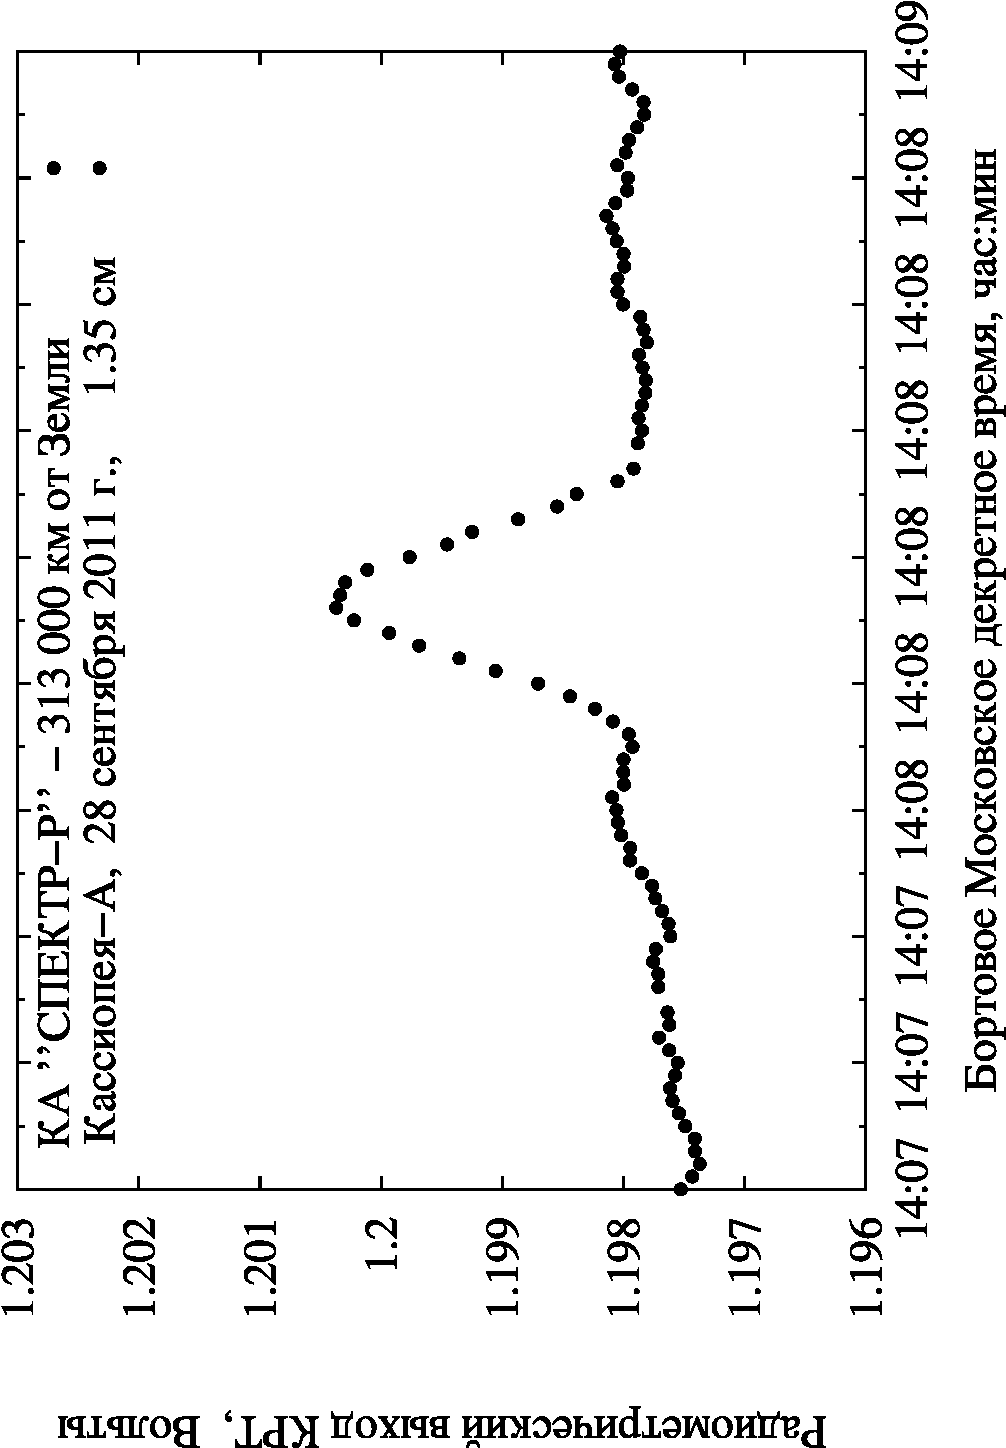
\includegraphics[width=0.3\textwidth,origin=c,angle=-90]{Fig8a_ru.pdf} \\
    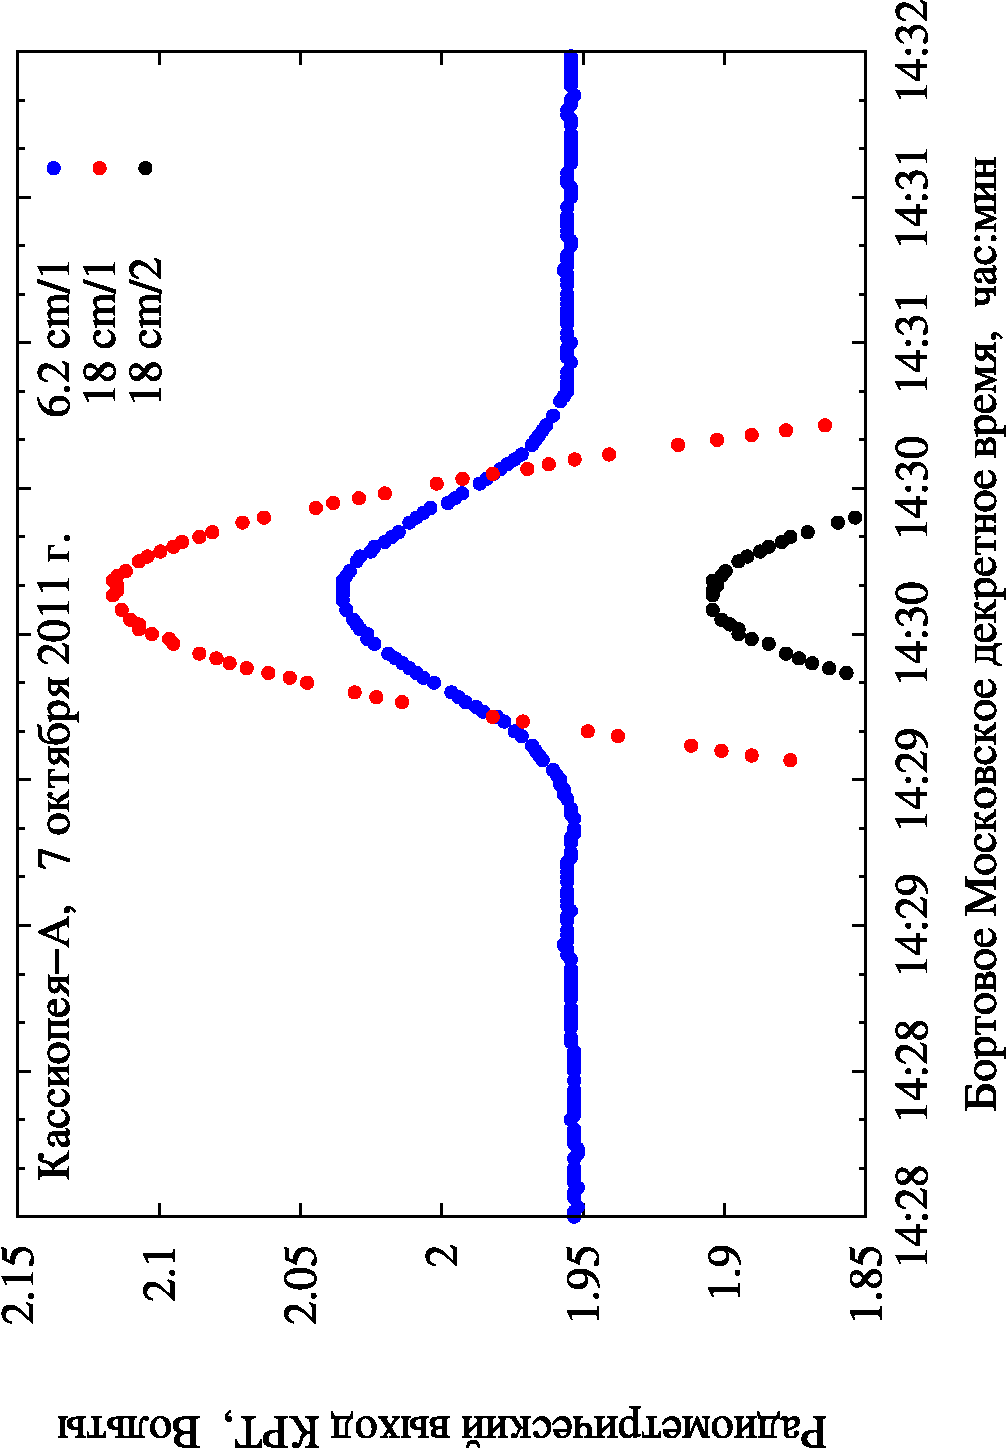
\includegraphics[width=0.3\textwidth,origin=c,angle=-90]{Fig8b_ru.pdf} \\
    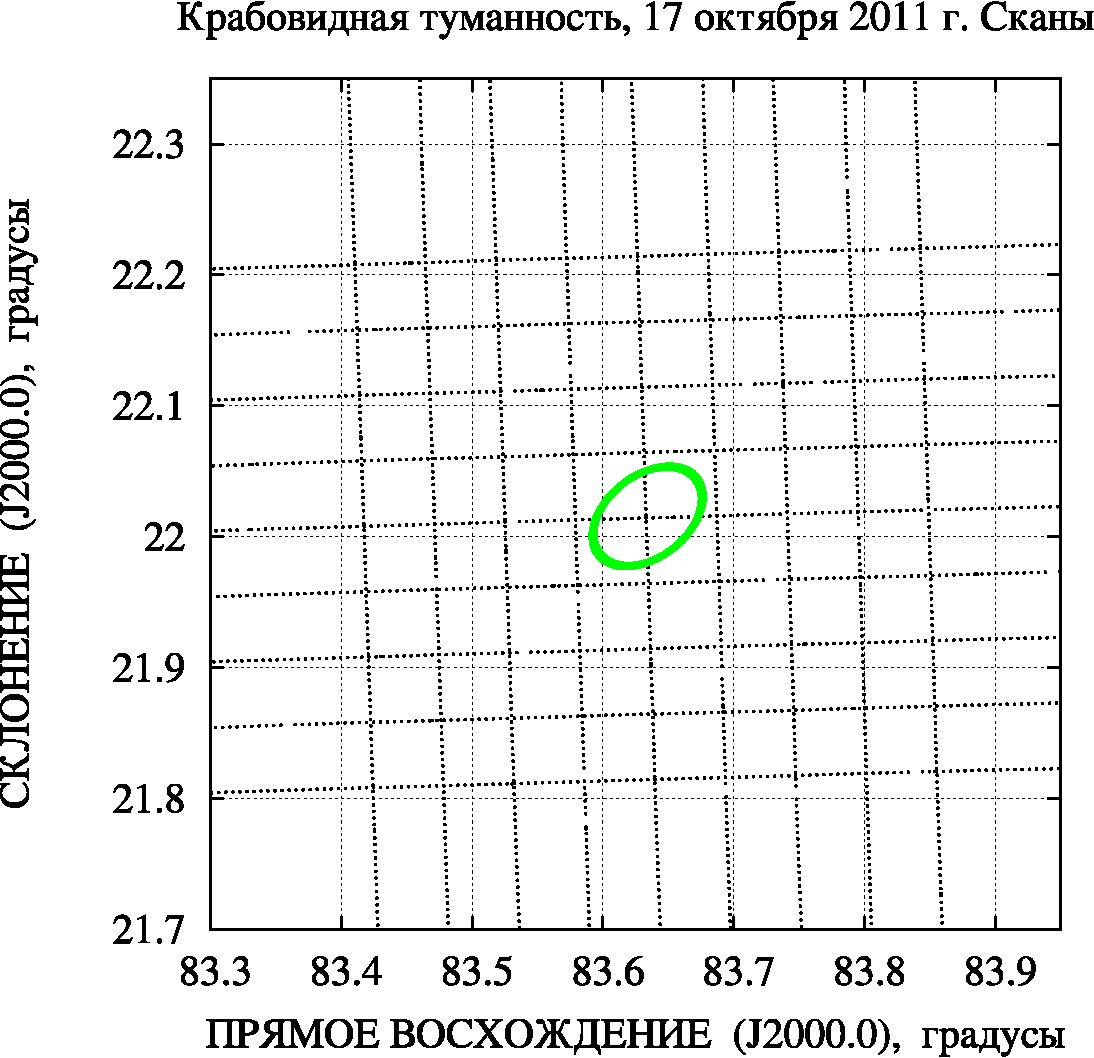
\includegraphics[width=0.3\textwidth,origin=c,angle=0]{Fig8c_ru.pdf}
 }
 \caption{Первый радиометрический отклик КРТ по наблюдениям Кассиопеи-А
в диапазоне 1.35 см 28 сентября 2011 г. (а)
и в диапазоне 6.2 см 7 октября 2011 г.
на фоне одновременных откликов в ортогональных поляризациях
на длине волны 18 см  (б).
Траектории сканирования участка неба с Крабовидной туманностью
17 октября 2011 г. (в), которым соответствуют отклики
сигналов в диапазонах 1.35 и 6.2 см, приведенные на графике 7б цветной вкладки.
Условный контур в центре характеризует угловые размеры
радиоисточника.}
\end{figure}

\begin{figure}[tbh]
 \centerfloat{
    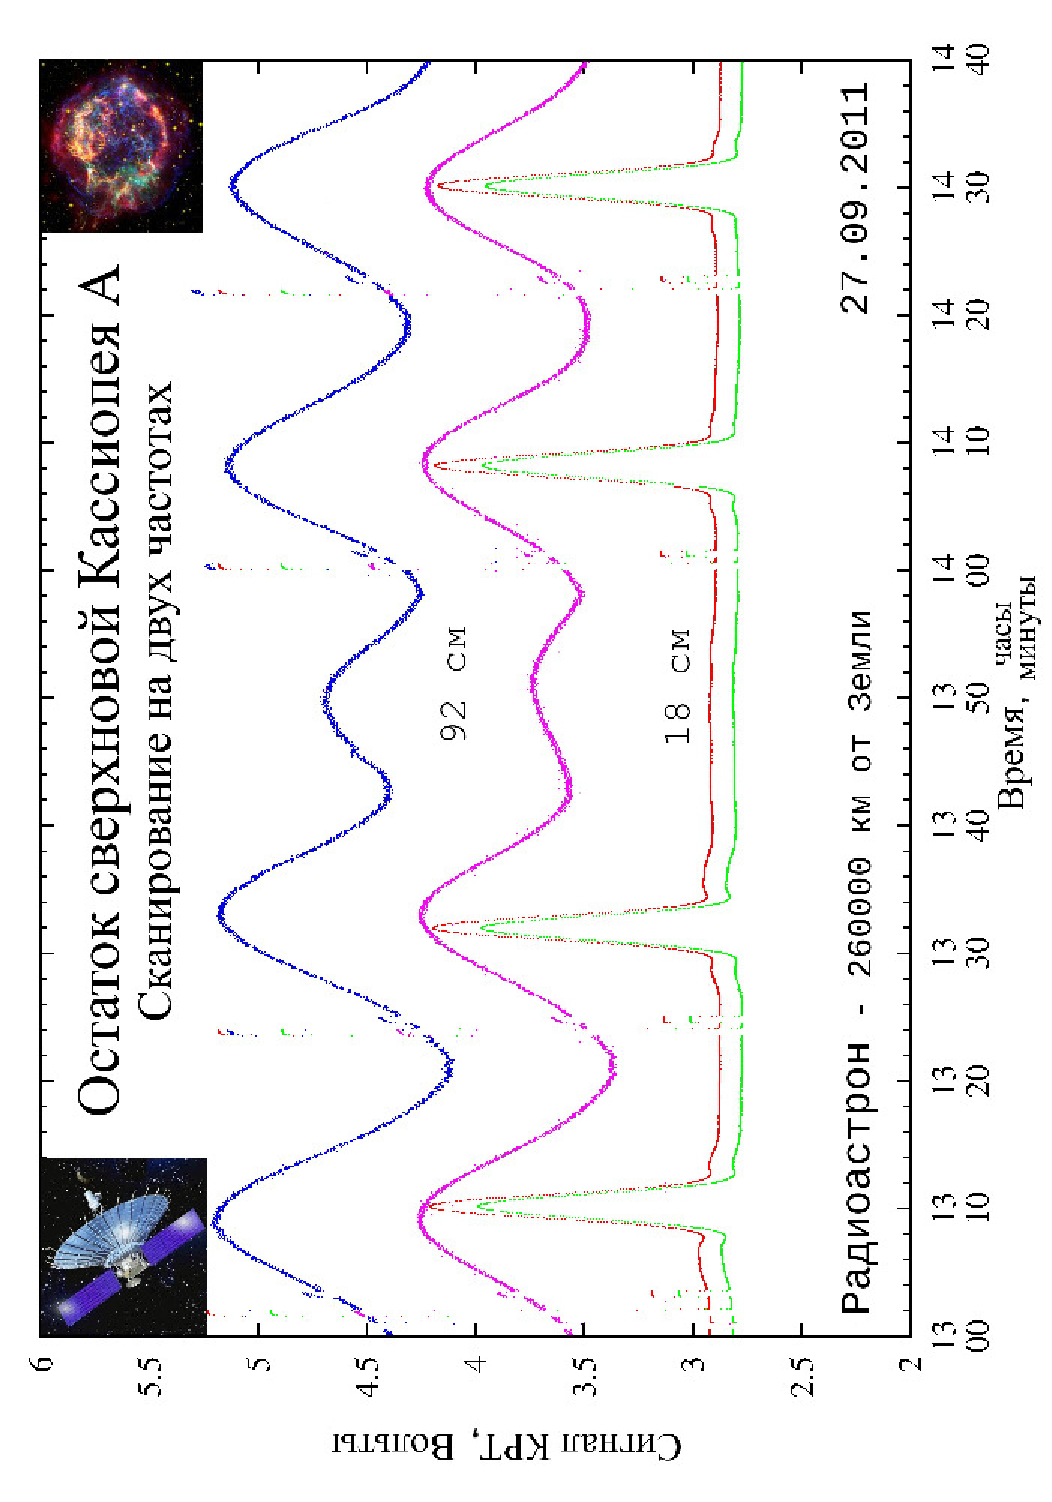
\includegraphics[width=0.3\textwidth,origin=c,angle=-90]{Fig7a_ru.pdf}
    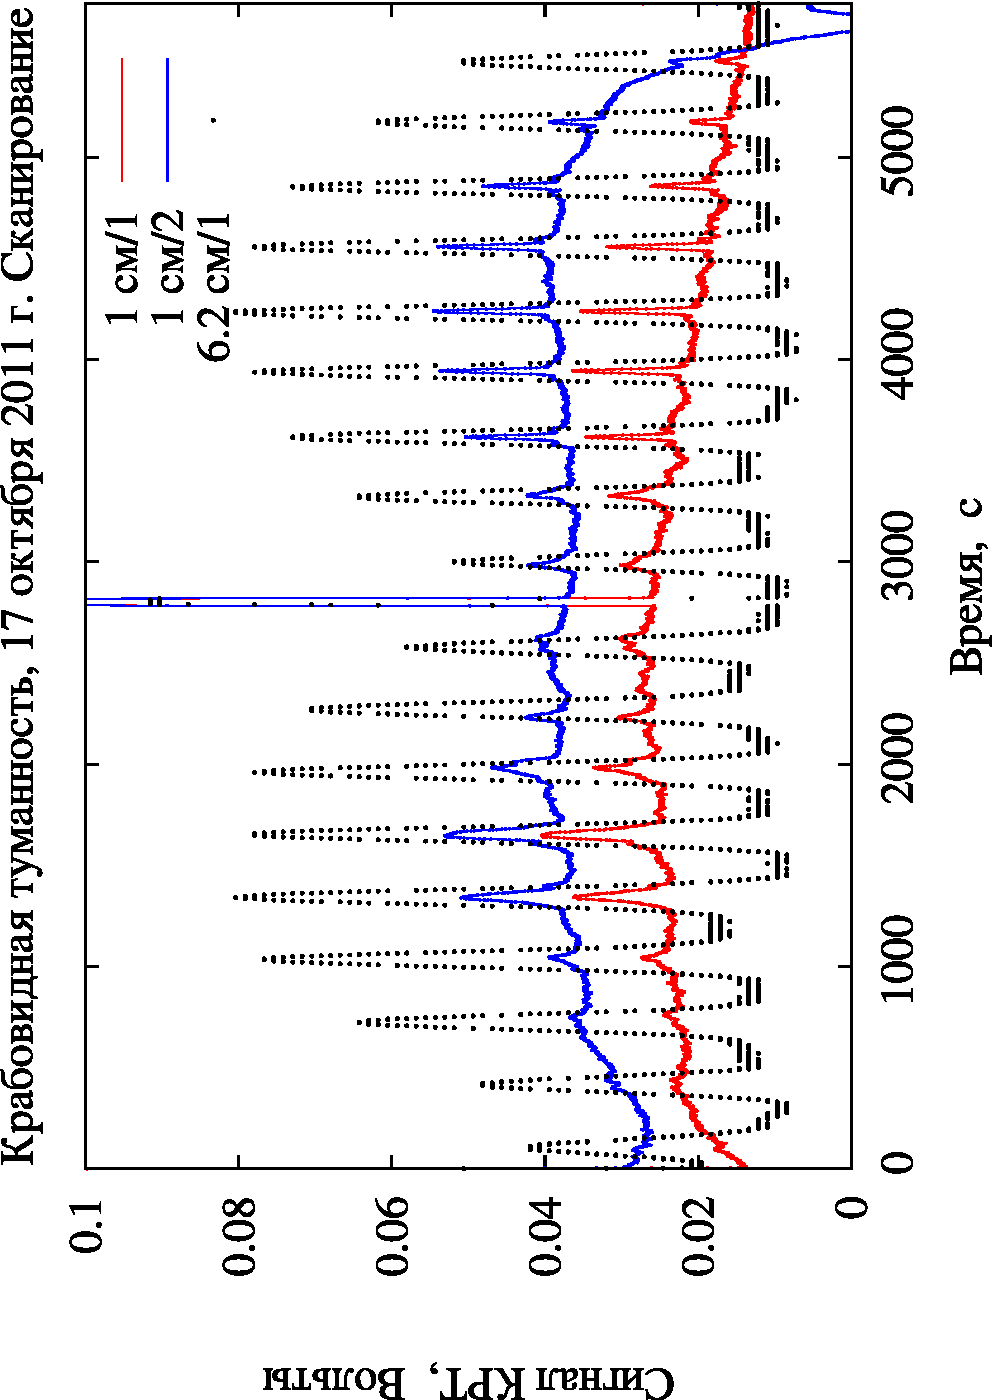
\includegraphics[width=0.3\textwidth,origin=c,angle=-90]{Fig7b_ru.pdf}
 }
 \caption{}
\end{figure}

\begin{figure}[tbh]
 \centerfloat{
    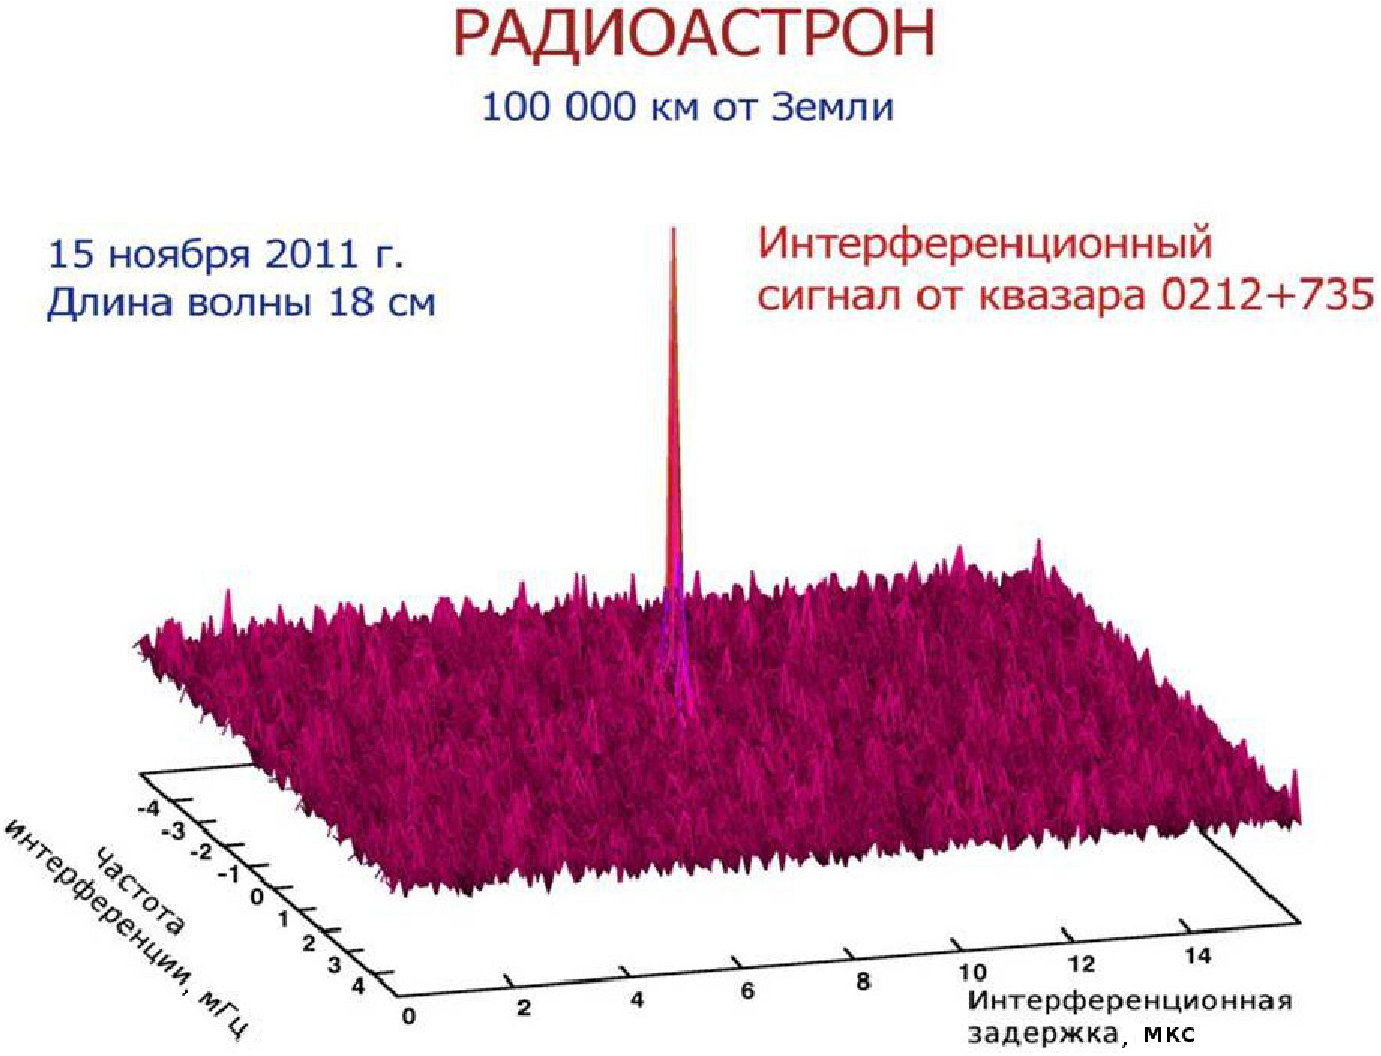
\includegraphics[width=0.4\textwidth]{Fig7c_ru.pdf} \hfill
    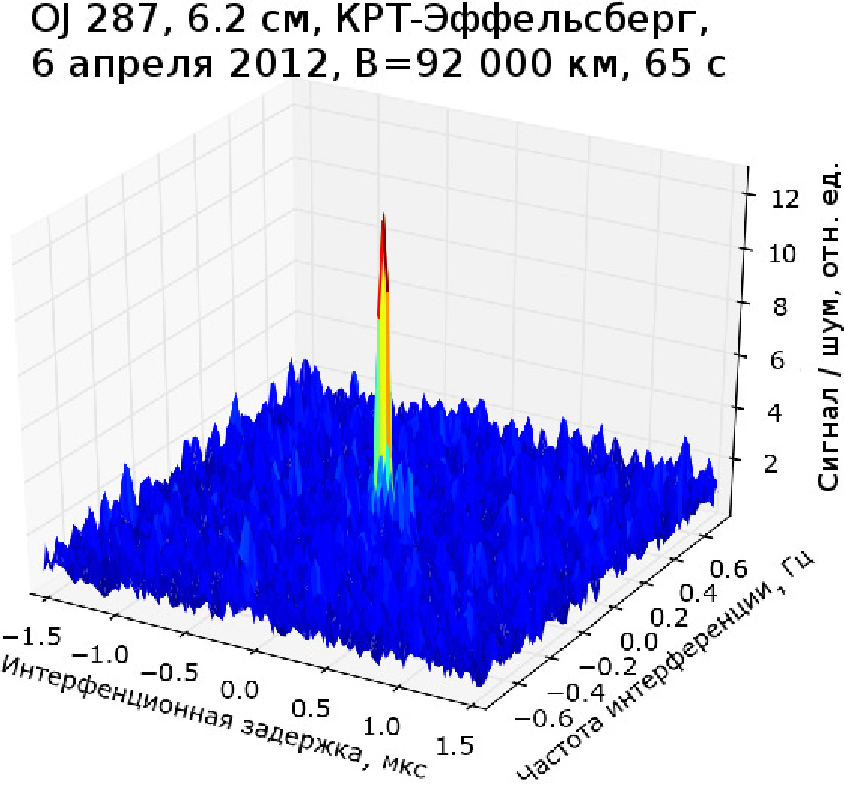
\includegraphics[width=0.4\textwidth]{Fig7d_ru.pdf}
 }
 \caption{}
\end{figure}

\begin{table}[tbh]
\caption{Основные ожидаемые (1.1--1.10) и измеренные
(2.1--2.10) параметры КРТ в диапазонах длин волн K, C, L, P:
ширина главного лепестка диаграммы направленности по уровню
половинной мощности $\vartheta_{0.5}$ и $\varphi_{0.5}$,
эффективная площадь $A_{eff}$,
коэффициент использования площади КИП,
эффективная температура шума системы $T_{sys}$ и приемника
$T_{rec}$,
эффективная плотность потока излучения системы $F_{sys} \equiv$ SEFD,
систематическая ошибка при сканировании  $\Delta \vartheta_s$
по оси $\vartheta$ и $\Delta \varphi_s$ по оси $\varphi$
после ввода постоянной поправки $\delta \vartheta_p$ в
наведение телескопа,
чувствительность интерферометра $\sigma_{SVLBI}$,
отношение $\alpha_{D}$
измеренной ширины главного лепестка диаграммы направленности к его
идеальной ширине $\lambda / D$, где $D = 10$ м --- диаметр зеркала}
\bigskip
\label{tab:srt_params1}
\centering
    \begin{SingleSpace}
        \begin{tabular}{l|r|r|r|r}
        % \hline
        \toprule
        Параметр              &K($1.35$ см)&C($6.2$ см)&L($18$ см)&P($92$ см)\\
        \midrule
1.\quad  КРТ в Пущино, 2003--2004:& & & &\\
                                  & & & &\\
1.1\quad $\vartheta_{0.5} \pm 5\%$, \,\,\,\,\,\,\,\,\,
&  $5.6^\prime$ & $25.5^\prime$  & $74.5^\prime$ & $6.2^\circ$ \\
1.2\quad  $A_{eff} \pm 10\%$, \,\,\,\,  м$^2$     &   27 &   40 &   40 &  24\\
1.3\quad  КИП = $A_{eff}/A_{geom} \pm 10\%$ & 0.34 & 0.51 & 0.51 & 0.31\\
1.4\quad  $T_{sys}/T_{rec}$, \,\,\, K                                   &80/45 & 70/30 & 50/15
&140/30\\
1.5\quad  $T_{sys}^{(opt)}$, \,\,\, K                                    &70    & 66    &  33  &
164\\
1.6\quad  $SEFD_{srt}^{(opt)}$, \,\,\, Ян                                        &7200    &4600
&2300  &19000\\
1.7\quad  $SEFD_{GB}$, \,\,\, Ян                                         & 23     & 8     & 10   &
55\\
1.8\quad  $\Delta \nu_{IF}$, \,\,\, МГц                                   & 16     & 16    & 16   &
4\\
1.9\quad  $\sigma_{SVLBI}^{(opt)}$ (при $\Delta t = 5$ мин), \,\,\, мЯн  & 7   & 3   & 3   & 33\\
1.10\quad  $\alpha_D = \vartheta_{0.5} \cdot D / \lambda$\,\,\,                     & 1.21   & 1.20
& 1.20 & 1.18\\
%[4pt]
\hline
%[-6pt]
2.\quad  КРТ в полете, 2011--2012: & & & &\\
                       & & & &\\
2.1\quad  $(\vartheta_{0.5} \pm 5 \%)$ x $(\varphi_{0.5} \pm 5 \%)$,\,
& $6.0^\prime$ x $13^\prime$ & $25^\prime$    & $72^\prime$   & $6.1^\circ$ \\
2.2\quad  $A_{eff} \pm 13\%$, \,\,\, м$^2$;                            & 7.5       & 35    & 41   &
30\\
2.3\quad  КИП = $A_{eff}/A_{geom} \pm 13\%$                            & 0.1       & 0.45  & 0.52 &
0.38\\
2.4\quad  $T_{sys} \pm 13\%$, \,\,\,\,\, K                             & 77        & 130   & 45   &
200\\
2.5\quad  $F_{sys} \pm 10\%$\,\,(SEFD$_{srt})$, \,\,\, Ян              & 30000 & 10500 & 3400 &
19000\\
2.6\quad  $\vert \Delta \vartheta_s \vert$, \,\,\,\, &$1.2^\prime \pm 0.2^\prime$            & & &
\\
2.7\quad  $\vert \Delta \varphi_s \vert$, \,\,\,\,\, &$< 1.5^\prime$            & & & \\
2.8\quad  $\delta \vartheta_p$, \,\,\,\,\,           &$2.5^\prime$              & & & \\
2.9\quad  $\sigma_{SVLBI}$ (при $\Delta t = 5$ мин), \,\,\, мЯн        & 13        & 5     & 3    &
33\\
2.10\quad  $\alpha_D = (\vartheta_{0.5}\times \varphi_{0.5}) \cdot D / \lambda$ &$1.29 \times 2.80$
&1.17 &1.16 &1.16\\
        \bottomrule
        \end{tabular}
    \end{SingleSpace}
\end{table}


%\vspace{1cm}
%{\it 5.5. Результаты}
%\vspace{0.5cm}
\subsubsection{Результаты}


Основные результаты суммированы в табл.~2 (измерения), а также в табл.~3 (анализ измерений) в
Приложении. В табл.~2 включены также основные результаты наземных радиоастрономических испытаний
технологической модели КРТ на полигоне в Пущинской обсерватории АКЦ ФИАН, полученные в 2003--2004
гг. \cite{SRT_report_2004}. Типичные радиометрические отклики на примерах первых сканирований
показаны на рис. 7a (цветная вкладка), 8a и 8б для диапазонов 92, 18, 1.35 и 6.2 см по наблюдениям
Кассиопеи-А (первого из астрономических объектов, наблюдавшихся с космическим радиотелескопом с 27
сентября 2011 г.) и на рис. 7б (цветная вкладка) по наблюдениям Крабовидной туманности в диапазонах
1.35 и 6.2 см. Пример сканирования площадки неба дан на рис. 8в. Приведенным на нем траекториям
соответствуют радиометрические отклики на рис. 7б. Для антенных измерений использовались также
Юпитер, Луна и Дева-A (протяженные объекты) и квазиточечные внегалактические радиоисточники 3С\,84,
3С\,273 и 3С\,279.

Характеристики  стандартных калибраторов (потоки, распределение яркости, угловые размеры,
поляризация) брались из литературы \cite{Baars_1977}, а потоки сильных квазиточечных радиоисточников
3С\,84, 3С\,273 и 3С\,279, являющихся переменными, --- по измерениям на 600-м кольцевом
радиотелескопе РАТАН-600 САО РАН (Нижний Архыз, Россия) и на 100-м параболоиде в Эффельсберге
Института радиоастрономии им. Макса Планка (Бонн, ФРГ) \cite{} в близкие к бортовым
измерениям даты. Процедуру наземных измерений см. в \cite{Kovalev_1999}.


%{\it 5.6. Обсуждение результатов}
%\vspace{0.5cm}
\subsubsection{Обсуждение результатов}

Как известно, при отсутствии фазовых погрешностей, ширина $\vartheta_{0.5}$ главного лепестка
диаграммы направленности по половинной мощности и коэффициент использования площади $\eta$ (КИП),
равный отношению эффективной площади к геометрической, зависят от закона распределения амплитуды и
фазы электрического поля по раскрыву зеркала антенны и от уровня облучения края зеркала. Для
идеального параболического рефлектора с диаметром $D$ круглого раскрыва, при некоторых типовых
теоретических законах амплитудного распределения синфазного поля, ожидаемые ширина диаграммы
$\vartheta_{0.5}$ и КИП $\eta_0$ на длине волны $\lambda$ для синфазного случая могут быть оценены с
помощью соотношений \cite{Hansen_1966,Ajzenberg_1977,Christiansen_1972} $\vartheta_{0.5} = \alpha_D
\cdot \lambda / D$, где $\alpha_D \approx 1.0 \div 1.5$, и $\eta_0 \approx 1.0 \div 0.55$ в
зависимости от конкретого закона распределения поля. При этом, чем меньше уровень облучения края
зеркала, тем меньше $\eta_0$ (КИП) и больше $\alpha_D$ (шире диаграмма направленности), и они близки
к единице только при одинаковой амплитуде поля по раскрыву. Фазовые искажения синфазного поля в
раскрыве дополнительно увеличивают коэффициент $\alpha_D$ и уменьшают $\eta_0$, т.е. расширяют
главный лепесток диаграммы направленности и уменьшают эффективную площадь.

Сравнивая эти значения $\alpha_D$ с полученными $\alpha_D \approx 1.2$ по измерениям КРТ (см.
параметры 1.10 и 2.10 в табл. 2), видим, что для диапазонов 92, 18 и 6.2 см измеренная ширина
главного лепестка диаграммы направленности соответствует значениям, близким к теоретически
ожидаемым. Наиболее существенные отличия результатов измерений параметров КРТ в полете от параметров
проектных или ожидаемых, полученных ранее по испытаниям КРТ в Пущино \cite{SRT_report_2004},
относятся к эффективной площади и к форме главного лепестка диаграммы направленности в диапазоне
1.35 см, а также к температуре шумов КРТ в диапазоне 6.2 см (табл.~2). Для работы в режиме синтеза
широкой полосы частот в диапазоне 1.35 см предусмотрен выбор любой из 8 входных полос. Приведенные
результаты относятся к центральной полосе $F_0$ (см. раздел 2.2.2).

%\vspace{0.5cm}
%{\it 5.6.1. Диапазон 1.35 см (центральная полоса F0)}
%\vspace{0.5cm}
\paragraph{Диапазон 1.35 см (центральная полоса $F_0$)}

Измеренное в этом диапазоне поперечное сечение главного лепестка диаграммы направленности по уровню
половинной мощности представляет собой примерно эллипс с осями $\vartheta_{0.5}\times \varphi_{0.5}$
= $6.0^\prime\times 13^\prime$ при относительной ошибке 5\%, вместо ожидаемого круга диаметром
$(5.6^\prime \pm 10\%)$. Наглядно эта особенность хорошо видна по откликам на сканирование площадки
неба с источником (рис. 7б на цветной вкладке и рис. 8в). Измеренная эффективная площадь оказалась
равной $(7.5 \pm 13\%)$ м$^2$ вместо ожидаемого значения $(27 \pm 10\%)$ м$^2$ или хотя бы
проектного значения $(23 \pm 15\%)$ м$^2$. Эти ожидаемые значения для диаграммы и площади были
получены при наземных испытаниях КРТ в Пущино в 2004 г. Отличие полученной в наземных испытаниях
эффективной площади от эффективной площади идеальной параболической поверхности ($40 \div 45$ м$^2$)
естественно объяснялось влиянием случайной погрешности реализации поверхности зеркала, выполненной
со среднеквадратичным отклонением не хуже проектного значения $\sigma = 0.77$ мм, которое было
задано в проекте допуском $d = \pm 2$ мм ($\vert d \vert = 2.6 \sigma$ \cite{Esepkina_1973}). Этой
же причиной, но при $\sigma \approx 1.4$ мм, или другой типичной причиной (систематической
квадратичной фазовой погрешностью в раскрыве антенны, --- с максимальным значением $\sim 1.5\,\pi$;
см. Приложение) могло бы быть формально объяснено и уменьшение эффективной площади до 7.5 м$^2$,
если бы не наблюдаемое при этом существенное искажение формы главного лепестка диаграммы
направленности.

Искажения диаграммы направленности в параболических антеннах вызываются, в основном, тремя видами
систематических фазовых искажений амплитудно-фазового распределения поля в раскрыве зеркала
\cite{Hansen_1966,Ajzenberg_1977,Christiansen_1972,Galimov_2010}: квадратичными, кубическими (комой)
и астигматизмом зеркала и/или облучателя. За квадратичные и кубические искажения могут быть
ответственны как зеркало или облучатель, так и смещение облучателя из фокуса зеркала --- в
продольном (для квадратичных искажений) или поперечном (для комы) направлениях к оси параболоида.
Астигматизм является следствием того факта, что точки наилучшей фокусировки в двух главных
взаимно-ортогональных плоскостях, перпендикулярных раскрыву, не совпадают \cite{Hansen_1966}. Это
означает, что оптимальная точка фокусировки для облучателя, установленного в положение с
минимальными аберрациями (и соответственно --- с минимальной шириной главного лепестка диаграммы
направленности), различна в этих плоскостях --- в каждой из них своя точка, и единый фазовый центр
отсутствует. При этом обычно существует некоторый общий <<эквивалентный центр оптимальной
фокусировки>> или <<эквивалентный фазовый центр>> вблизи середины этих положений, при установке в
который фазовые аберрации и искажения диаграммы направленности удается минимизировать
\cite{Hansen_1966,Galimov_2010}. Фазовые погрешности в раскрыве есть сумма всех погрешностей,
обусловленных зеркалом, облучателем и смещением облучателя из фокуса зеркала
\cite{Shubarin_1960,Cejtlin_1976}. Поэтому однозначно установить реальную причину фазовых искажений
в раскрыве антенны только по результатам летных испытаний, без дополнительных данных или
предположений, не представляется возможным.

Как свидетельствует подробный анализ проблемы (см. Приложение), наблюдаемую эллиптичность главного
лепестка диаграммы направленности, как и измеренное значение эффективной площади, в диапазоне 1.35
см проще всего объяснить, предположив систематическую квадратичную погрешность в распределении фазы
по оси $\varphi$ порядка $1.5 \pi$ в раскрыве антенны и астигматизм, обусловленные облучателем,
дополнительно к случайной погрешности реализации параболической поверхности зеркала КРТ с проектным
значением среднеквадратичного отклонения $\sigma = 0.77$ мм, использованным выше. Такая
систематическая фазовая погрешность по одной оси в раскрыве могла бы, например, возникать при
астигматизме облучателя с квадратичной фазовой погрешностью и одновременном смещении центра
оптимальной фокусировки облучателя относительно фокуса зеркала на величину порядка 0.3 см вдоль оси
параболоида, при расстоянии $b \sim 2$ см между двумя такими центрами фокусировки облучателя. В
пользу этого предположения свидетельствуют результаты оценок в одной из моделей фазовых искажений в
Приложении, использующей результаты численного расчета \cite{}  амплитудно-фазовой диаграммы
направленности БАО. Расчет \cite{} указывает на возможность астигматизма и квадратичных аберраций
облучения зеркала со значениями, близкими к необходимым для объяснения результатов измерений в
диапазоне 1.35 см.

Предпринятые попытки (см. Приложение) дать согласованное аргументированное объяснение всей
совокупности антенных измерений без астигматизма облучателя в этом диапазоне успеха не имели. Но это
только одно из возможных объяснений. Формально можно также предположить, что полученные
систематические фазовые погрешности в раскрыве вызваны не облучателем, а зеркалом антенны. Однако
для такого вывода в настоящий момент нет достаточных оснований и данных для количественного анализа.
Простой близкий вариант для объяснения асимметрии диаграммы направленности --- гипотеза о
соответствующей сильной асимметричной деформации зеркала --- так, чтобы размер раскрыва антенны в
одной из плоскостей уменьшился примерно вдвое (до 5 м), должен был бы сказаться на результатах во
всех диапазонах. А это противоречит <<хорошим>> результатам антенных измерений в диапазонах 6.2, 18
и 92 см, которые близки к проектным.

%\vspace{0.5cm}
%{\it 5.6.2. Диапазоны 6 см, 18 см и 92 см}
%\vspace{0.5cm}
\paragraph{Диапазоны 6.2, 18 и 92 см}

В отличие от других диапазонов все измерения в диапазоне 6.2 см проведены при раздельной работе с
поляризационными каналами. Одновременное их включение сразу приводило к зашкалу выходных сигналов,
которое не устранялось аттенюаторами. Зарегистрированы также искажения автоспектра выходных
видеополос для канала с правой поляризацией в интерферометрическом режиме. Эти факты позволяют
предположить, что на участке <<вход БАО--вход МШУ>> антенно-фидерного тракта в диапазоне 6.2 см
ухудшилось согласование поляризационных каналов БАО со свободным пространством и/или с МШУ и
ухудшилась развязка между каналами. Это привело к увеличению реактивных и активных потерь на этом
участке при раздельном включении каналов и, как следствие, к увеличению шумовой температуры системы
согласно (5.7), а также к самовозбуждению МШУ при одновременной работе каналов. Исследование
продолжается.

Во всех антенных измерениях использовались предварительные значения антенной температуры $T_{NS}$
ГШ, полученные по результатам предполетных наземных измерений и <<пересчета>> $T_{NS}$ ко входу КРТ
согласно формуле (5.7в) по измеренным или рассчитанным потерям  \cite{RAUH} в антенно-фидерном
тракте. Планировалась их коррекция по результатам летных испытаний. Коррекция для диапазонов 92, 18
и 1.35 см не проводилась. Коррекция $T_{NS}$ ГШ для диапазона 6.2 см проведена: 1) в предположении
соответствующего увеличения потерь в БАО (т.е. уменьшения $K_2$ в соотношениях (5.7б), (5.7в)) и 2)
в пренебрежении искажениями от диаграммы направленности облучателя, уменьшающими эффективную
площадь, что не противоречит результатам расчета  \cite{} и оценкам параметров 4.2 и 5.2 в табл.~3
для этого диапазона\footnote {Так как в блоке антенных облучателей (БАО) конструктивно объединены
облучатели с полосковыми или волноводными формирователями левой и правой круговых поляризаций для
каждого дипапазона (см. разделы 5.1 и  2), то потери в БАО характеризуют не только потери в самих
облучателях (в основном, на высшие типы волн), но и в следующих за ними поляризаторах. }. Эта
коррекция привела к соответствующему увеличению полученных значений эффективной площади $A_{eff}$ и
эквивалентной шумовой температуры системы $T_{sys}$ в диапазоне 6.2 см (т.е. к <<улучшению>>
$A_{eff}$ и <<ухудшению>> $T_{sys}$).

Она же  позволила дать общее согласованное объяснение измеренной зависимости эффективной площади КРТ
от длины волны во всех диапазонах с помощью единого подхода к учету фазовых погрешностей. И
одновременно --- объяснить соответствующее повышение шумовой температуры системы согласно (5.7)  в
диапазоне 6.2 см и, возможно, частично, в диапазоне 92 см: увеличением потерь $L_2$ в БАО
относительно проектных значений\footnote {Из-за недостатка средств  и известных технических проблем
калибровки антенных измерений, в том числе и проблем изготовления высококачественных апертурных
охлаждаемых согласованных нагрузок, проектная документация содержит только расчетное значение потерь
БАО в диапазоне 92 см и результаты косвенных лабораторных измерений  или теоретических оценок таких
потерь в остальных диапазонах.}. Для шумовой температуры КРТ в диапазоне 92 см существенен также
вклад от фонового излучения неба, который, кроме того, может заметно меняться с изменением
направления на объект и полностью или частично объяснять 20-процентное превышение измеренной
температуры шумов КРТ $T_{sys} = 200$ К над ожидаемой. Минимальный вклад фона неба при антенне,
направленной в полюс Галактики, по оценкам, использующим опубликованные распределения яркостной
температуры неба и соотношения (5.7), (5.7а), составляет около 60 К, который включен в ожидаемую
температуру $T_{sys}^{(opt)} = 164 $ К \cite{RAUH}.

Стоит подчеркнуть, что потери $L_2 = 1 / K_2$ БАО входят в 3 слагаемых в (5.7), что не всегда
принимается во внимание при грубых оценках. Заметим также, что, в отличие от калибровки по антенной
температуре, необходимой для антенных измерений, обычно используемая в астрономических измерениях
<<астрономическая калибровка>> наземных радиотелескопов и КРТ, --- в единицах эквивалентной
спектральной плотности потока излучения для системы с помощью $F_{sys}$ (SEFD) и для генератора шума
ГШ  с помощью $F_{NS}$,   --- не зависит от этих особенностей и коррекций, так как пропорциональна
$T_{sys}/A_{eff}$ (для SEFD) или $T_{NS} / A_{eff}$ (для $F_{NS}$), и может выполняться по
астрономическим источникам радиоизлучения без знания абсолютных величин антенной температуры
$T_{NS}$ ГШ и $T_{sys}$ системы (см. раздел 5.1 и \cite{Kovalev_1999}).

%\vspace{0.5cm}
%{\it 5.6.3. Поправки наведения и сканирования}
%\vspace{0.5cm}
\paragraph{Поправки наведения и сканирования}

Поправки измерялись при сканировании площадки с источником
по осям $\vartheta$ и $\varphi$ (см. пример на рис. 7б на цветной вкладке и рис. 8в).
По результатам такого сканирования находились центральные
сечения источника, для которых процесс сканирования многократно
повторялся в прямом и обратном направлениях движения по каждой оси.
Используя телеметрические данные штатного координатного обеспечения,
отдельно для прямого и для обратного направлений сканы
усреднялись, и вычислялась разность координат между расчетным и
измеренным положениями максимума сигнала, которая и определяла
искомые поправки к расчетным координатам.

Измеренная величина погрешности координат по оси $\vartheta$ (с меньшей шириной
диаграммы направленности, равной $\vartheta_{0.5} = 6^\prime$)
при сканировании <<вперед>> систематически отличается от величины
при сканировании <<назад>>, а кривая сканирования имеет характерный для наземных
телескопов <<двугорбый>> вид  со значениями, равными $(3.7^\prime \pm 0.2^\prime)$
для одного максимума и $ 1.3^\prime \pm 0.2^\prime $    для другого максимума.
По этим данным введена постоянная поправка в наведение
$\Delta \vartheta_p = 2.5^\prime$,
равная среднему значению между ними, с которой далее  работали постоянно.
"Двугорбость>> при сканировании в противоположных направлениях сохранялась,
--- примерно с прежним запаздыванием, соответствующим
$\vert \Delta \vartheta_s \vert = 1.2^\prime \pm 0.2^\prime$ к расчетному значению, ---
всегда с запаздыванием по времени, независимо от прямого или обратного
направления сканирования, но уже относительно нулевого среднего значения
между максимумами. Такое запаздывание электрической оси при движении КРТ
относительно нового расчетного положения оси мы интерпретировали как
систематическую ошибку сканирования (табл.~2).
По другой оси поправка не вводилась, так как результаты
были в пределах ошибок измерений.

Примерно половина измеренного интервала времени между <<горбами>> может объясняться эффектом
задержки отклика при интегрировании сигнала на радиометрическом выходе (см. об этом эффекте в
\cite{Kuzmin_1964}). Считается, что основная причина двугорбой кривой для наземных телескопов
(отсутствующая для КРТ) --- люфты в механизмах управления. Причина аналогичного поведения КРТ может
быть связана с подобными задержками при интегрировании сигналов в электронике систем звездных
датчиков и цепях управления движением космического аппарата или с другими причинами и нуждается в
дополнительном изучении. Гипотезе об упругих деформациях штанг, на которых крепится фокальный
контейнер КРТ, противоречат результаты анализа телеметрии, свидетельствующие о достаточно
равномерной скорости на участках движения.

%\vspace{0.5cm}
%{\it 5.6.4. Шум телеметрии}
%\vspace{0.5cm}
\paragraph{Шум телеметрии}

Анализ телеметрических данных показал наличие дополнительного
<<шума телеметрии>> для цифровых радиометрических выходов в обоих каналах
приемников диапазонов 18 и 92 см.
Он имеет вид фона, состоящего из <<пачек>> коротких импульсных
выбросов, и характерен для ошибок регистрации отдельных бит: амплитуда их
<<переменности>> не случайна, а систематически повторяется, изменяясь дискретно
от <<пачки к пачке>>. Сравнение с телеметрируемым параметром приемников <<АЦП готов>>
позволяет предположить, что этот шум вызван тем, что штатная телеметрическая система,
осуществляя опрос всех датчиков с фиксированной скоростью, не учитывает сигнал
готовности аналого-цифрового преобразователя (АЦП) в приемниках.
В результате опрос цифровых датчиков иногда осуществляется быстрее
реальной готовности АЦП в этих приборах. Впервые такой шум был обнаружен в
процессе приемо-сдаточных испытаний. Был найден и применен простой и эффективный
способ фильтрации, использование которого позволило устранить эту проблему
и в антенных измерениях КРТ в полете. В аналоговых выходах этих диапазонов
и во всех выходах приемников двух других диапазонов такой шум отсутствует.


\subsubsection{Выводы}

1. Полученная эквивалентная температура шума системы КРТ в пределах 20\%
совпадает с теоретическими оценкам в диапазонах 92, 18 и 1.35 см,
но вдвое превышает расчетное значение в диапазоне 6.2 см, что
в $\sqrt 2$ раз снижает ожидавшуюся для этого диапазона
чувствительность интерферометра (при фиксированном времени накопления).
Причиной такого повышения температуры шума, вероятно, является увеличение потерь в
антенно-фидерном тракте (скорее всего, на участке от БАО до МШУ) по сравнению с
потерями, рассчитанными на основе лабораторных измерений, выполненных на Земле.


2. Ширина главного лепестка диграммы направленности КРТ по уровню половинной мощности
в пределах погрешности близка к теоретически ожидаемым
и измеренным в наземных испытаниях значениям в
диапазонах 92, 18 и 6.2 см,
но заметно отличается от таковых в диапазоне 1.35 см:
поперечное сечение главного лепестка по уровню половинной мощности
на длине волны 1.35 см близко к эллиптическому с осями
$\vartheta_{0.5} \approx 6.0^\prime \pm 5\%$ и
$\varphi_{0.5} \approx 13 ^\prime  \pm 5\%$
 вместо проектной окружности диаметром $5.5 ^\prime  \pm 10\%$.
При этом профиль продольного сечения главного лепестка в той плоскости,
где он шире, заметно асимметричен.

3. Эффективная площадь КРТ в полете близка к расчетной или измеренной в наземных
испытаниях в диапазонах 92, 18 и 6.2 см.
В диапазоне 1.35 см она меньше ожидаемой по наземным измерениям площади
($27 \pm 10\%$) м$^2$ в 3.6 раза и проектной площади ($23 \pm 15\%$) м$^2$ ---
втрое, что почти в 2 раза уменьшает ожидаемую чувствительность в
интерферометрическом режиме (при фиксированном времени накопления).

4. Оценки, выполненные на основе расчетных значений амплитудно-фазовой диаграммы
направленности блока антенных облучателей  и простой модели фазовых погрешностей
в антенно-фидерной системе, приводят к следующим выводам о КРТ в полете:

--- средний профиль поверхности зеркала антенны может быть близким к
 параболическому с проектным значением  среднеквадратичного отклонения
 реальной поверхности зеркала от средней, равным 0.77 мм;

---  облучатель антенны может иметь:
а) квадратичные фазовые погрешности с максимальным значением
погрешности фазы облучения края зеркала, равным примерно $-100^\circ$ в
диапазоне 1.35 см и $-35^\circ$ в диапазонах 6.2 и 18 см
(согласно расчетным значениям фазовой диаграммы направленности
этих облучателей);
б) астигматические аберрации в диапазоне 1.35 см, аппроксимируемые
двумя эквивалентными центрами фокусировки облучателя, --- центрами 1 и 2
в ортогональных плоскостях 1 и 2, соответственно,---
вынесенными из фокуса зеркала примерно на 7 мм к зеркалу в
плоскости 1 и на 13 мм от зеркала в плоскости 2;
в) общий центр оптимальной фокусировки облучателя
(середина между центрами 1 и 2), который вынесен из фокуса
раскрывшейся антенны примерно на 3 мм от
зеркала в продольном направлении оси антенны;

--- эти фазовые погрешности облучения поверхности зеркала антенны
могут быть основными причинами измеренного уменьшения эффективной
площади и эллиптичности главного лепестка диаграммы направленности
КРТ в диапазоне 1.35 см  относительно проектных значений.

5. По результатам радиоюстировки средние погрешности наведения по
одной оси (с меньшей шириной главного лепестка диаграммы направленности
КРТ) составили $3.7^\prime \pm 0.2^\prime$  при
сканировании источника в одном направлении и $1.3^\prime \pm 0.2^\prime$  при сканировании в
противоположном направлении.
Частично этот результат может объясняться эффектом запаздывания отклика
из-за интегрирования
сигнала на радиометрическом выходе и нуждается в дополнительном изучении.
По этим измерениям введена постоянная поправка наведения
$\Delta \vartheta_p = 2.5^\prime$,
с которой далее работали постоянно. Оставшаяся погрешность сканирования
$\vert \Delta \vartheta_s \vert = 1.2^\prime \pm 0.2^\prime$   характеризует
запаздывание максимума сигнала относительно его расчетного
положения при сканировании в любом направлении и вызвана систематичеcкой
погрешностью при движении антенны.
По другой оси (с большей шириной главного лепестка диаграммы) погрешность
наведения лежит в пределах точности измерений, не превышая $1.5^\prime$,
и не компенсировалась в дальнейших наблюдениях.

6. Сравнение автокорреляционных спектров двух сильных мазерных источников в
диапазонах L и K позволяет сделать вывод о штатном функционировании спектрального
режима наблюдений космическим радиотелескопом и позволяет контролировать
частотные настройки и режимы поляризации при наблюдениях. Оценки чувствительности
КРТ, проведенные в рамках наблюдений спектральных радиолиний, согласуются
с данными исследований по источникам непрерывного спектра.
Незавершенной остается задача полного определения поляризационных параметров
радиотелескопа, что возможно при специально запланированных наблюдениях нескольких
ярких источников мазерного излучения, в частности, Orion KL.


\subsection{ПРОВЕРКА ФУНКЦИОНИРОВАНИЯ НАЗЕМНО-КОСМИЧЕСКОГО
         ИНТЕРФЕРОМЕТРА (ПЕРВЫЕ ЛЕПЕСТКИ) И ПЕРВЫЕ РЕЗУЛЬТАТЫ
         НАБЛЮДЕНИЙ}

В данном разделе представлен краткий обзор первых результатов,
полученных в интерферометрическом режиме. Эти результаты
будут подробнее обсуждаться в отдельных статьях позднее,
международными группами по поиску лепестков и Ранней научной
программе после завершения всестороннего анализа.

Детектирование интерференционного сигнала между космической обсерваторией
<<РадиоАстрон>>
и наземными радиотелескопами продемонстрировало общую успешную работу
комплексной РСДБ системы <<Космос--Земля>> во всех четырех диапазонах длин волн:
92, 18, 6.2 и 1.35 см (рис. 7в--7ж на цветной вкладке).
Первый сигнал космического
интерферометра был получен по наблюдениям 15 ноября 2011 г. квазара 0212+735 в
диапазоне 18 см при удалении КА от Земли, составившим около 100 000 км,
и проекции базы <<РадиоАстрон>> -- 100-м радиотелескоп в Эффельсберге
(Германия) на картинную плоскость источника $B = 8100$ км (рис. 7в на цветной вкладке).
Всего ко времени написания статьи проведено 20 сеансов испытаний интерферометра.
На рекордном удалении КА в 300 000 км (проекция базы составила
около 220 000 км) 25 января 2012 г. были проведены интерферометрические
наблюдения пульсара PSR 0950+08 в диапазоне 92 см с участием самого крупного
наземного радиотелескопа диаметром 300 м в обсерватории Аресибо (США) (рис. 7е, 7ж на цветной
вкладке).
Большинство
интерферометрических наблюдений проводилось в режиме c бортовым водородным
мазером, но были выполнены и успешные сеансы испытаний интерферометра в режиме
передачи на космический аппарат когерентного сигнала от водородного стандарта
Станции слежения в Пущино с обратной передачей его с аппарата на Станцию слежения
(так называемый <<режим замкнутой фазовой петли>>).

В режиме интерферометра чувствительность системы двух телескопов
пропорциональна квадратному корню из произведения эффективной
площади этих телескопов, и, таким образом, сочетание 10-м КРТ со 100-м
наземным радиотелескопом становится эквивалентным по чувствительности
системе двух 30-м телескопов. Режим наземно-космического
интерферометра не позволяет
получать результат исследования сразу после проведения измерений.
Зарегистрированные на различных радиотелескопах научные данные
передаются в центр обработки для первичной корреляции (обнаружения
интерферометрического отклика). Эта первичная корреляция может быть
выполнена только после высокоточной реконструкции орбиты КА в
баллистическом центре.

Обработка и анализ результатов, полученных на наземно-космическом интерферометре <<РадиоАстрон>>,
производится в АКЦ ФИАН совместно с другими участниками проекта. Здесь, в первую очередь,
выполняется кросс-корреляционная обработка потоков данных, записанных на отдельных радиотелескопах с
плотностью записи 128 или 256 Мбит/с, включая космический сегмент КРТ (128 Мбит/с), с помощью
созданной в АКЦ ФИАН системы регистрации РДР-1 \cite{Belousov_2007} и регистратора Mark5
\cite{Whitney_2003} разработки США. Программный FX-коррелятор АКЦ ФИАН построен на базе
вычислительного кластера с производительностью 1 Тфлоп/с и RAID-системой хранения информации
емкостью до 220 Тбайт. Технические характеристики процессорного кластера ЦОНИ АКЦ ФИАН позволяют
принимать поток данных от 10 станций, включая КРТ, с интегральной скоростью до 2.56 Гбит/с и,
соответственно, обрабатывать потоки до 45 формируемых в эксперименте баз интерферометров. Это может
выполняться практически без снижения темпа записанных в реальном времени и сохраненных в ЦОНИ данных
наблюдений.

Само по себе обнаружение интерферометрического отклика ещё не является окончательным результатом
научного исследования. Однако, при определенных предположениях о структуре компактной детали, оно
позволяет оценить ее угловой размер и яркостную температуру. Для достоверного заключения о строении
исследуемого объекта необходимы многократные наблюдения с различными конфигурациями телескопов и,
прежде всего, --- при разных положениях космического аппарата на его орбите. Необходимый набор таких
конфигураций может быть реализован как минимум в течение одного календарного года. Стратегия
наблюдений состоит в исследовании определенной выборки радиоисточников в течение целого года (а
иногда и нескольких лет), после чего всесторонний анализ дает возможность сделать обоснованные
заключения о структуре и физических условиях в изучаемых космических объектах.

Ранняя научная программа <<РадиоАстрон>> курируется АКЦ ФИАН и проводится с февраля 2012 г.
международными коллективами исследователей, сформированными в рамках проекта. К настоящему времени
измерены интерферометрические отклики от пульсаров PSR 0950+08, PSR 0531+21 (Crab) и PSR 0833-45
(Vela), PSR 1919+21, от активных ядер галактик 0212+735, 0716+714, 0748+126, 0754+100, 2013+370,
0851+202 (OJ287), 1954+513, 2200+420 (BL Lac), от галактического мазера W51 (см. Информационные
сообщения проекта <<РадиоАстрон>> за 2011--2012 гг. \cite{RA_news}). Эти отклики получены для
проекций базы наземно-космического интерферометра на картинную плоскость исследуемого источника
размерами от менее 10 000 км до около 250 000 км, т.е. примерно до 20 диаметров Земли.

14 ноября 2011 г., после подтверждения наблюдаемости на КРТ гигантских радиоимпульсов от пульсара в
Крабовидной туманности (расстояние 1 кпк), в диапазоне 18~см была впервые найдена корреляция между
этими импульсами, зарегистрированными КРТ и наземными радиотелескопами в Евпатории и обсерваториях
<<Светлое>>, <<Зеленчукская>> и <<Бадары>> ИПА РАН при проекциях базы интерферометров на картинную
плоскость источника до $B = 40 000$ км (рис. 10). Этот факт свидетельствует о том, что рассеяния
изображения в межзвездной среде от пульсара до наблюдателя на длине волны 18 см было не более
углового разрешения интерферометра, которое составило 400 мксек. дуги.

Интерферометрические наблюдения обычных импульсов близкого (260 пк) пульсара PSR 0950+08 (рис. 7е на
цветной вкладке) не обнаружили межзвездного рассеяния изображения даже в диапазоне 92 см при
проекции базы интерферометра вплоть до $B=220 000$ км. Тем самым впервые практически в метровом
диапазоне длин волн достигнуто угловое разрешение в  370 мксек. дуги. Наблюдения того же пульсара в
течении 1 ч (рис. 7ж на цветной вкладке) позволили впервые обнаружить переменность функции видности
интерферометра при столь больших базах интерферометра, что открывает путь к изучению параметров
турбулентности межзвездной плазмы и достижению еще более высокого углового разрешения источника с
использованием принципа <<межзёздного интерферометра>> \cite{Wolszczan_1987}. Для другого близкого
пульсара Vela, расстояние до которого $\sim 300$ пк, рассеяние в межзвездной среде было
зафиксировано. В мае 2012~г. крупнейшие радиотелескопы южного полушария провели совместно с КРТ
наблюдения этого пульсара на волне 18 см. В этих наблюдениях участвовали радиотелескопы обсерваторий
Паркс, Мопра, Хоббарт (все Австралия) и Хартбизтхоук (ЮАР), а также антенна НАСА в Тидбинбилла
(Австралия). Обработка данных показала, что при проекции базы в 100 000 км полностью изменяется
структура интерференционного отклика (наблюдается множество узких всплесков), что указывает на
многолучевое распространение радиоволн через неоднородную межзвёздную плазму.

Пример отклика источника мазерного излучения молекулы H$_2$O (диапазон 1.35 см) из области
звездообразования W51, полученный при наблюдении на радиоинтерферометре КРТ --- 100-м  радиотелескоп
в Эффельсберге (Германия), представлен на рис. 7д (цветная вкладка). Наблюдения проводились 12 мая
2012 г., проекция базы наземно-космического интерферометра составила 14 500 км (1.14 диаметра
Земли), что обеспечило на этой длине волны угловое разрешение в 80 мксек.\,дуги.

Наибольшее количество интерферометрических наблюдений было связано с изучением структуры ядер
активных галактик. Для двух квазаров, OJ 287 (c двойной чёрной дырой в центре, как предполагается
некоторыми авторами --- см., например, \cite{Valtonen_2011}) и BL~Lacertae (прототип объектов класса
лацертид), получены интерференционные отклики при наблюдениях в диапазоне 6.2 см с проекцией базы
КРТ--Эффельсберг, равной $B = 7.2$ диаметра Земли, или 92 000~км. Это позволяет оценить величину
яркостной температуры для доминирующей детали в излучении компактной струи\,--\,ядра: около или
более $10^{13}$ К. Это больше, чем известный комптоновский предел \cite{Kellermann_1969} на
яркостную температуру, но излучение все еще может объясняться в рамках стандартной модели
некогерентного синхротронного излучения струи релятивистских электронов, усиленного за счет эффекта
Доплера \cite{Cohen_2007}.

Для активной галактики 0716+714 --- одного из самых быстропеременных внегалактических объектов ---
успешное детектирование интерференционных лепестков в том же диапазоне было выполнено для многих
проекций баз, от примерно 1.5 до более 5 диаметров Земли. Международной рабочей группе по Ранней
научной программе проекта <<РадиоАстрон>> удалось по этим данным восстановить изображение объекта
(рис. 11) и измерить параметры видимого ядра. Ширина у основания струи в ядре объекта оказалась
равной примерно 70 мксек. дуги или 0.3 пк, а яркостная температура --- $2 \cdot 10^{12}$~K. Заметим,
что эти параметры измерены в момент минимума активности этого объекта.

\begin{figure}[tbh]
 \centerfloat{
  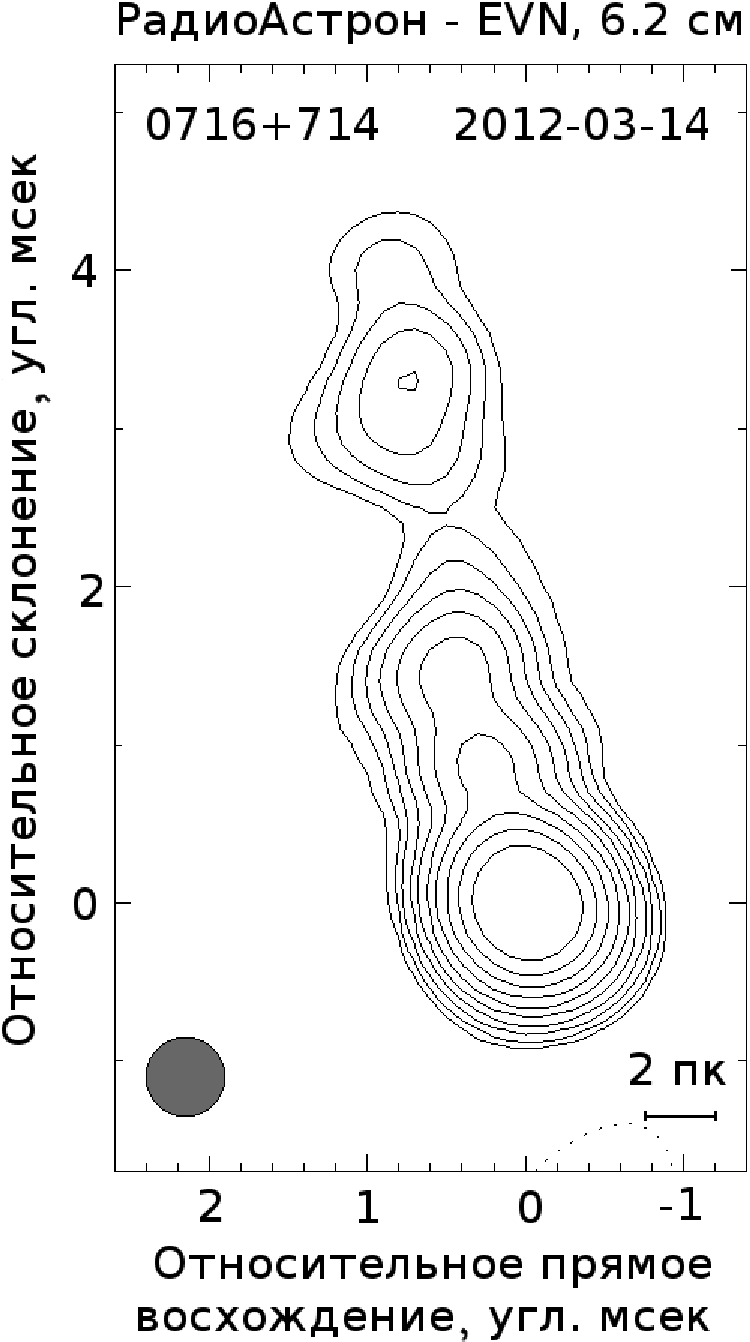
\includegraphics[scale=0.5]{map_0716+714.pdf}
 }
 \caption{Изображение быстропеременного объекта типа BL Lacertae 0716+714, полученное
по данным на длине волны 6.2 см. Наблюдения проведены совместно КРТ и Европейской
РСДБ-сетью 14--15 марта 2012 г. в рамках Ранней научной программы проекта
<<РадиоАстрон>> по активным ядрам галактик. Карта восстановлена
с использованием диаграммы направленности шириной 0.5 мсек. дуги
по уровню половинной мощности, сечение которой показано в левом нижнем углу
рисунка.  Контуры проведены по уровню равной интенсивности с
возрастанием в два раза для каждого следующего уровня, начиная с 0.25 мЯн/луч.
Интенсивность в максимуме равна 0.43 Ян/луч. <<Луч>> (<<beam>>) есть телесный
угол показанного сечения.}
 \label{fig:map_0716}
\end{figure}


\section{Измерение и анализ основных параметров космического телескопа <<РадиоАстрон>> в полете в
2011--2013 гг.}

\subsection{Введение}

Описание КА Спектр-Р, космического радиотелескопа (КРТ), научной аппаратуры и наземных испытаний
даны в \cite{Khartov_2011,Alexandrov_2011a,Alexandrov_2011b}. Результаты летных испытаний, методика
и первые результаты антенных измерений основных параметров телескопа радиоастрономическими методами
в радиометричесом режиме для диапазонов 92, 18, 6.2 и 1.35 см приведены в
\cite{Avdeev_2012,Kardashev_2013_rus,RAUH} --- для эффективной площади, шумовой температуры,
диаграммы направленности, погрешности наведения на источник и др.

В данной статье сообщается о новых результатах периодического контроля основных
антеных параметров, полученных в течение 2011--2013 гг. Измерения выполнены  как
в специальных сеансах наблюдений известных общепринятых первичных калибровочных
астрономических объектов, так и в процессе текущих сеансов массовых научных
наблюдений в режиме наземно-космического радиоинтерферометра со сверхбольшой
базой (РСДБ) --- как часть данных, требующихся для калибровки РСДБ наблюдений по
спектральной плотности потока излучения при выполнении Ранней научной программы
исследований.

Впервые представлены результаты антенных измерений в 8 поддиапазонах интервала частот 18--25 ГГц,
предназначенных для их использования в режиме многочастотного синтеза изображений в дальнейших
работах с РСДБ. Для калибровки этих измерений по потоку, кроме известных протяженных первичных
калибровочных источников (Кассиопея А, Лебедь А, Краб, Дева А), использовались также несколько
квазиточечных для КРТ сильных переменных внегалактических объектов (3С 84, 3С 273, 3C 279),
спектральные плотности потока излучения которых в близкие даты измерялись по известным вторичным
калибраторам на радиотелескопе РАТАН-600 Специальной астрофизической обсерватории РАН (Нижний Архыз,
Россия) и 100-м телескопе Института радиоастрономии общества Макса Планка (Эффельсберг, Германия).

\subsection{Измерения}

Измерения антенных параметров основаны на относительных измерениях эквивалентной спектральной
плотности потока шумового излучения системы $F_{sys}$ [Ян] (SEFD) --- относительно астрономических
калибраторов. Эквивалентная шумовая температура системы (радиотелескопа) $T_{sys}$ измерялась
относительно считающейся известной антенной температуры бортовых генераторов шумового сигнала (в
градусах К), входящих в состав каждого научного приемника.

Бортовой научный комплекс включает в себя 4 радиоастрономических супергетеродинных приемника --- на
диапазоны 92, 18, 6.2 и 1.35 см. Приемник диапазона 1.35 см обеспечивает также прием сигнала в 8
переключаемых поддиапазонах от 1.7 до 1.2 см с помощью выбора одного из поддиапазонов
соответствующими командами. Блоки входных малошумящих усилителей (МШУ) приемников всех диапазонов,
кроме 92 см, вынесены в открытый космос и размещены на <<холодной плите>>, охлаждаемой до
температуры 130 К радиационным способом. Каждый приемник состоит из 2-х идентичных каналов, на входы
которых от антенны через блок антенных облучателей (БАО) с разделителями поляризаций поступает
излучение в левой и правой круговых поляризациях. Каждый канал имеет два параллельных выхода: 1)
радиометрический выход --- с продетектированным сигналом, который поступает на телеметрическую
систему космического аппарата и используется в антенных измерениях, 2) интерферометрический выход
--- с сигналом на промежуточной частоте, который после дальнейших преобразований используется в
работе наземно-космического интерферометра.

Специальные сеансы наблюдений калибровочных объектов обычно проводились в режиме работы одиночного
телескопа. Тогда телеметрическая информация после буферной записи и хранения в бортовом
запоминающеем устройстве передавалась на Землю в течение суток через малонаправленную антенну по
служебному телеметрическому радиоканалу космического аппарата. При интерферометрических наблюдениях
исследуемых источников данные телеметрической системы последовательно размещаются в заголовках
каждого кадра потока данных для интерферометра и передаются на Землю в реальном времени через
остронаправленную антенну диаметром 1.5 м по научному высокоинформативному радиоканалу. Это дает
возможность выделять телеметрируемый радиометрический сигнал из интерферометрического потока данных
с КРТ. Таким путем в данной работе получены результаты антенных измерений по источникам, исследуемым
с интерферометром в научных программах.


\subsection{Обсуждение измерений}
\subsubsection{Диапазоны 92, 18, 6.2 и 1.35 см}

Анализ измерений показывает, что практически все основные антенные параметры иcпытывают вариации от
измерения к измерению, основную причину которых мы связывем с изменениями температурных условий
(соответствующих проектным), в которых находятся антенно-фидерный тракт и приемники. Физические
температуры элементов антенно-фидерного тракта и входных блоков МШУ приемников могут меняться из-за
изменений угла между направлениями на Солнце и объект измерения от сеанса к сеансу. Чем ближе этот
угол к проектной границе ($\approx 110^\circ$) допустимой работы КРТ, тем больших отклонений от
средних значений можно ожидать. При этом должен меняться и вклад в эквивалентную температуру системы
от потерь в антенных облучателях с разделителями поляриризаций, поэтому можно ожидать также заметных
вариаций эффективной температуры $T_{NS}$ калибровочного сигнала. Этот сигнал от внутреннего
шумового генератора поступает в тракт приемника на входе блока МШУ и приводится ко входу системы
телескопа, <<пересчитываясь>> через все элементы антенно-фидерного тракта.

Поэтому ниже для упрощения анализа предполагалось выполненным условие постоянства средних значений
$T_{NS}$ и  эффективной площади $A_{eff}$. Тогда все их реальные вариации автоматически относятся на
счет изменений $T_{sys}$. Заметим, что такая процедура не влияет на корректность <<астрономической
калибровки>> измерений с помощью параметра $F_{sys}$ (SEFD), зависящего от отношения $T_{sys} /
A_{eff}$. Обоснованием допустимости этого условия в данном случае могут служить приведенные ниже
результаты для среднеквадратичных отклонений $T_{sys}$ и $F_{sys}$ по калибровочным и исследуемым
источникам, которые не превышают примерно 13\%.

В пределах погрешности измерений полученные результаты для средних значений системной температуры
$T_{sys}$ и плотности потока $F_{sys}$ (SEFD) в диапазонах 92, 18, 6.2 и 1.35 см, с учетом
различного вклада вклада фона неба, согласуются как для калибровочных и исследуемых источников, так
и с первыми результатами, приведенными в работе \cite{Kardashev_2013_rus}: в пределах (20--25)\%
для диапазона 1.35 см и (10--15)\% для остальных диапазонов. Вместе с тем нельзя исключить, что
около половины от этих значений связана с медленной систематической эволюцией данных параметров,
включая их калибровку.

Заметный вклад в наблюдаемое рассеяние значений $T_{sys}$ относительно среднего может давать
изменение рассогласования МШУ с трактом <<БАО-вход МШУ>> и связанное с этим изменение коэффициента
шума МШУ, которые зависят от физических температур БАО и МШУ (развязки на входе МШУ, как обычно,
отсутствуют для понижения шумовой температуры приемника).

\subsubsection{Диапазон (18--25) ГГц}

Диапазон предназначен для использования в режиме многочастотного синтеза интерферометра и состоит из
8 следующих поддиапазонов (с указанными центральными частотами), отстоящих друг от друга на 960 МГц
\cite{Kardashev_2013_rus}: $F_{-4}$ (18392 МГц), $F_{-3}$ (19352 МГц), $F_{-2}$ (20312 МГц),
$F_{-1}$ (21272 МГц), $F_0$ (22232 МГц), $F_1$ (23192 МГц),  $F_2$ (24152 МГц), $F_3$ (25112 МГц)
--- см. рис. 3. Значения центральных частот могут быть на 4 МГц больше или меньше указанных, в
зависимости от заданного режима работы научной аппаратуры. Результаты измерений $F_{sys}$
($SEFD_{SRT}$) в этих поддиапазонах, приведенные на Рис.~3, и оценка чувствительности интерферометра
в Табл.~3 подтверждают теоретически ожидаемый монотонный <<ход>> $SEFD_{SRT}$ и чувствительности
интерферометра с ростом частоты, за исключением, быть может, их поведения на крайних частотах --
около 18 и 25 ГГц. Приведенные в табл.~3 чувствительности  рассчитаны по известной формуле
\cite{Kardashev_2013_rus}
\[
\sigma_{GBT-SRT} = b\, \sqrt{\frac {SEFD_{GBT}\, SEFD_{SRT}}{2\, \Delta \nu_{IF} \Delta t}},
\]
\noindent
где $b = 1/0.637$, $SEFD_{GBT} = \SI{23}{\jansky}$ (для радиотелескопа НРАО в Грин Бэнке), $\Delta
\nu_{IF} = \SI{16}{\MHz}$~"--- полоса регистрируемых частот, $\Delta t = 5$~мин~"--- время
интегрирования сигнала. В зависимости от режима работы интерферометра возможна также регистрация
сигнала в полосе $\Delta\nu_{IF} = \SI{32}{\MHz}$ \cite{Kardashev_2013_rus}. Значение
$\Delta\nu_{IF} = \SI{16}{\MHz}$ использовано для единообразия с \cite{RAUH}.

Из данных на рис. 3 и в табл. 3 следует возможность проведения интерферометрических измерений в этом
режиме в пяти длинноволновых поддиапазонах c $F_{-4}$ по $F_0$ c чувствительностью не ниже, чем в
$F_0$ на частоте 22 ГГц (длина волны 1.35 см). В трех коротковолновых поддиапазонах $F_1$, $F_2$ и
$F_3$ оцененная чувствительность может быть до полутора раз меньше, чем в $F_0$, из-за более
сильного вклада фазовых погрешностей на длинах волн меньше 1.35 см. Эта длина волны близка к так
называемой <<проектной минимальной длине волны использования телескопа>> $\lambda_{min} \equiv
(16\text{--}20)\sigma \approx 18\sigma= \SI{1.39}{\cm}$ при проектном значении $\sigma =
\SI{0.77}{\mm}$ (подробнее см. \cite{Esepkina_1973,Kuhn_1967,Cejtlin_1976} и разделы 3.2 и 3.3
ниже).

\begin{table}[tbh]
\caption{Результаты массовых измерений и расчетных оценок при наблюдениях калибровочных и
исследуемых источников в левой (LCP) и правой (RCP) круговых поляризациях в 2011--2013 гг.
\tiny{Примечание. Измерения калибраторов в диапазонах 1.35 и 6.2 см даны за 2011–2012 гг. Ошибки
шкалы спектральной плотности потока не включены. В строках 3.3–3.6 и 3.7 (3.10) даны оценки вкладов
в $T_{sys}$ от шумовых температур приемника $T_{rec}$, кабеля (волновода – в диапазоне 1.35 см)
$T_{Cable}$, блока антенных облучателей $T_{BAO}$, антенны $T_a$ и фона неба $T_{sky}$,
соответственно.
}}
\bigskip
\label{tab:srt_params2}
\centering
    \begin{SingleSpace}
    \tiny
        \begin{tabular}{lcccc}
        \toprule
Параметр              & 1.35 см  & 6.2 см   & 18 cм    & 92 см\\
                      & LCP; RCP & LCP; RCP & LCP; RCP & LCP; RCP\\

        \midrule
1 КАЛИБРАТОРЫ              & & & &\\
1.1 $T_{sys}$, K    & $98\pm13$; $82\pm11$    & $133\pm17$; --  &
$47.2\pm1.0$ ; $48.4\pm1.0$  & $230\pm5$; $210\pm11$ \\
1.2 $F_{sys}$, кЯн  & $36.0\pm3.6$; $30\pm3.0$ & $10.5\pm1.1$; -- & $3.18\pm0.06$; $3.26\pm0.07$
& $21.2\pm0.42$; $19.4\pm1.0$\\
2 ДРУГИЕ объекты         & & & &\\
2.1 $T_{sys}$, K    & $127\pm8$; $100\pm10$      & $147\pm8$; --  & $41.0\pm1.0$; $43.5\pm4.0$
& $145\pm15$; $147\pm15$\\
2.2 $F_{sys}$, кЯн  & $46.7\pm3.0$; $36.8\pm3.7$ & $11.6\pm0.63$; -- & $2.76\pm0.27$; $2.93\pm0.27$
& $13.3\pm1.4$; $13.5\pm1.4$\\
\midrule
3 РАСЧЕТ $T_{sys}$ и $F_{sys}$.& & & &\\
3.1 Коэффиц. передачи: & & & &\\
--- Kабеля $K_3/t_3$  &  0.99/157      & 0.94/157        & 0.95/157       & 0.98/233 \\
--- БАО $K_2/t_2$     &  0.76;0.84/175 & 0.68/175        & 0.95/175       & 0.83/175 \\
--- Aнтенны $K_1/t_1$ &  0.98/200      & 0.98/200        & 0.98/200       & 0.98/200 \\
3.2 $T_{rec} / t_4$, K   & 45 /140 & 26/140 & 15/140 & 39/290\\
3.3 $\Delta T_{rec}$, K  & 61; 55     & 42     & 17     & 49    \\
3.4 $\Delta T_{Cable}$, K&  2         & 15     & 8.9    &  6    \\
3.5 $\Delta T_{BAO}$, K  & 56; 34     & 84     & 9.4    & 36    \\
3.6 $\Delta T_A$, K      & 4          &  4     & 4      &  4    \\
3.7 $T_{sky}$, K         & 3          &  3     & 3      &  3+50 \\
3.8 $T_{sys}$, K         & 126; 98    & 148    & 42.3   &  98+50\\
3.9 $F_{sys}$, кЯн     & 46.4; 36.1& 11.7& 2.85   & 13.6  \\
Калибраторы: & & & & \\
3.10 $T_{sky}$, K         &    --       &  --     & $3+5$    &  $3+120$  \\
3.11 $T_{sys}$, К         &    --       &  --     & $42.3+5$ &  $98+120$ \\
3.12 $F_{sys}$, кЯн       &    --       &  --     & $3.18$   &  $19.5$    \\
        \bottomrule
        \end{tabular}
    \end{SingleSpace}
\end{table}

\begin{table}[tbh]
\caption{Основные параметры КРТ по \cite{Kardashev_2013_rus} и новым измерениям.
\tiny{Примечание. В строках 1--11 даны: ширина главного лепестка диаграммы направленности по уровню
половинной мощности --- 1, эффективная площадь --- 2, коэффициент использования площади --- 3,
эквивалентная температура шума и плотность потока шумового излучения системы --- 4 и 5, усиление
телескопа --- 6, систематическая погрешность при сканировании площадки неба
по двум координатам (строки 7 и 8) после ввода постоянной поправки (строка 9) в наведение телескопа,
чувствительность интерферометра КРТ – Green Bank Telescope по (1) и [6] --- 10, отношение
измеренной ширины к идеальной ширине $\lambda/\text{D}$ главного лепестка диаграммы направленности
--- 11.}}
\bigskip
\label{tab:srt_params3}
\centering
    \begin{SingleSpace}
    \tiny
        \begin{tabular}{lcccc}
        \toprule
Параметр              & 1.35 см  & 6.2 см   & 18 cм    & 92 см\\
                      & LCP; RCP & LCP; RCP & LCP; RCP & LCP; RCP\\

        \midrule
КРТ в полете, 2011--2013: & & & &\\
                       & & & &\\
1. $(\vartheta_{0.5} \pm 5 \%) \times (\varphi_{0.5} \pm 5 \%)$ & $6.0' \times 13'$ & $25'$ &$72'$
 & $6^\circ.1$ \\
2. $A_{eff} \pm 10\%$, м$^2$                  & 7.5        & 35     & 41         & 30\\
3. КИП = $A_{eff}/A_{geom} \pm 10\%$          & 0.1        & 0.45   & 0.52       & 0.38\\
4. $T_{sys} \pm 10\%$, K                      & 127; 100   & 147;  -- & 41.0; 43.5 & 145; 147\\
5. $F_{sys} \pm 10\%$ (SEFD), кЯн             & 46.7; 36.8 & 11.6; --& 2.76; 2.93 & 13.3;13.5\\
5. Усиление, Ян/K                             & 368        &  78.9  & 67.3       & 92.0     \\
6. $\Delta \vartheta_s$  & $-1.2' \pm 0.2'$    & & & \\
7. $\Delta \varphi_s$    & $< 1.5'$            & & & \\
8. $\delta \varphi_p$    & $2.5'$              & & & \\
9. $\sigma_{SVLBI}$, мЯн          & 17; 15 &  5; --  & 3; 3    & 14; 14\\
   (при $\Delta t = 5$ мин; $\Delta \nu = 16$ Мгц)            &        &        &         &
\\
10. $\alpha_D = (\vartheta_{0.5} \times \varphi_{0.5}) \cdot D / \lambda$ &  1.29 x 2.80 & 1.17 &
1.16 & 1.16\\
        \bottomrule
        \end{tabular}
    \end{SingleSpace}
\end{table}

\subsection{Заключение}

Новые результаты радиометрических измерений параметров космического радиотелескопа в 2011–2013 годах
по калибровочным объектам с помощью одиночного КРТ и по большому количеству исследуемых источников в
режиме интерферометра согласуются с первыми результатами, полученными Кардашевым и др. [5], --- в
пределах (10--15)\% в диапазонах 92, 18 и 6.2 см и (20--25)\% в диапазоне 1.35 см.

Основной вклад в SEFD и чувствительность КРТ в диапазонах 92, 18 и 6.2 см вносят шумы приемника и
блока антенных облучателей, а в диапазоне 1.35 см – потери эффективной площади из-за фазовых
погрешностей в антенно-фидерной системе. Вклад КРТ в чувствительность наземно-космического
интерферометра, пропорциональный корню квадратному из измеренных значений SEFD, близок к проектному
в диапазонах 92 и 18 см и уменьшает проектную чувствительность примерно в 1.5 и 2 раза в диапазонах
6.2 и 1.35 см, соответственно. Измеренный вклад КРТ увеличивает чувствительность интерферометра до
1.5 раз в 5-ти поддиапазонах на частотах от 22 до 18 ГГц и уменьшает ее до 1.5 раз в 3-х
поддиапазонах на частотах от 22 до 25 ГГц относительно чувствительности на 22 ГГц.

Основной вклад в эквивалентную шумовую температуру КРТ вносят приемник и блок антенных облучателей
(БАО) с разделителями поляризаций. Разброс значений этой шумовой температуры, через зависимость от
физических температур МШУ и БАО, может быть связан с изменениями ориентации КРТ относительно Солнца
в индивидуальных сеансах наблюдений.

Полученные результаты и опыт эксплуатации КРТ могут быть полезны при разработке будущих космических
проектов (<<Миллиметрон>> и др.; особенно учитывая, что антенна КРТ, вероятно, самая большая на
сегодня конструкция, раскрытая в космосе). Они указывают на необходимость проектной оптимизации
фазовых погрешностей поверхности и облучения зеркала и минимизации потерь как в отдельных элементах,
так и в антенно-фидерной системе с приемниками в целом. Для уменьшения фазовых искажений вблизи
минимальной длины волны использования телескопа может оказаться целесообразным дополнительное
проектное недооблучение края зеркала, уменьшающее известный оптимальный уровень в несколько раз.


\section{RadioAstron space VLBI imaging of polarized radio emission in the high-redshift quasar
0642+449 at 1.6 GHz}

\subsection{Подгонка лепестков}

Подгонка интерференционных лепестков проходила в два этапа: сначала применялась ручная коррекция
фазы, а затем использовался глобальный поиск лепестков для определения частоты интерференции на
антеннах и одно и многополосные задержки. Также была исправлена разность групповых задержек между
каналами поляризации. Полученные значения частоты интерференции для наземно-космических баз
представлены на рис.~\ref{fig:0642_rate}. Эта плавно меняющаяся остаточная частота
хорошо согласуется с ожидаемой точность определения орбитальной скорости КРТ
\cite{Kardashev_2013_rus}, но всё же она должна
рассматриваться только как индикатор качества данных, в то время как более подробное обсуждение
точности восстановления орбиты КРТ представлено в работе \cite{Duev_2015}.

\begin{figure}[tbh]
 \centerfloat{
  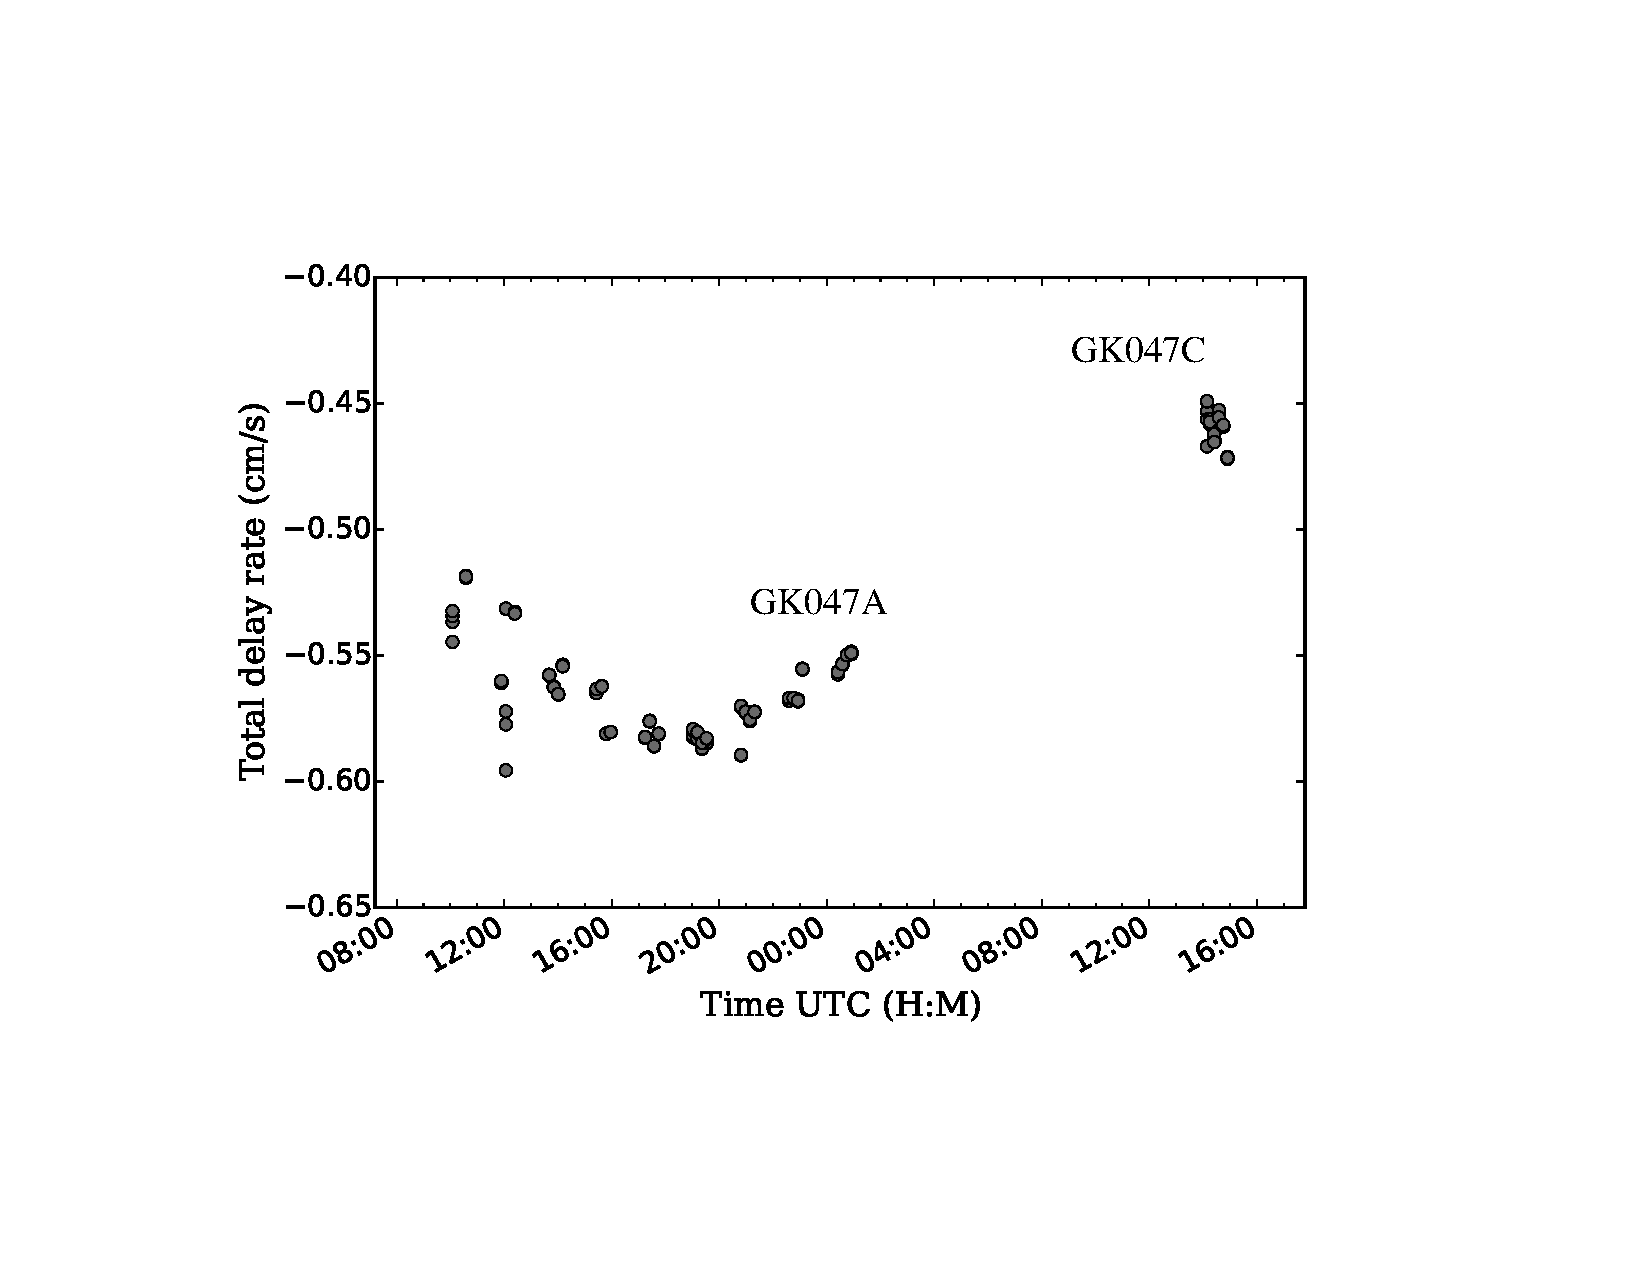
\includegraphics[width=0.9\textwidth]{totalrate.pdf}
 }
 \caption{Полная частота интерференции, полученная из подгонки лепестков на базе КРТ-Эффельсберг и
включающая в себя изменение хода часов каждого из телескопов. Для каждого наблюдательного сегмента
КРТ была получена частота интерференции с помощью подгонки лепестков на временном интервале 10
минут. Частоты нарисованы отдельно для каждого частотного и поляризационного канала. Рисунок
отражает точность определения скорости при реконструкции орбиты КРТ. Все значения скорости и
ускорения являются проекциями истинный остаточных скорости и ускорения космического аппарата.}
 \label{fig:0642_rate}
\end{figure}


\section{RadioAstron orbit determination and evaluation of its results using correlation of
space-VLBI observations}

\subsection{Введение}

Космический аппарат РадиоАстрон, оснащенный 10-метровым космическим радиотелескопом (КРТ), был
запущен на высокоэллиптическую орбиту Земли в июле 2011 года с помощью ракеты <<Зенит-3Ф>> с
разгонным блоком <<Фрегат-СБ>>. Основное назначение космического аппарата --- проводить наблюдения
галактических и внегалактических радиоисточников вместе с наземными радиотелескопами, образуя
многоантенный наземный радиоинтерферометр с чрезвычайно длинными базами \cite{Kardashev_2013_rus}.
Космический аппарат также позволил проверить Принцип эквивалентности Эйнштейна благодаря его
эксцентричной орбите и высокостабильному бортовому водородному стандарту частоты
\cite{Litvinov_2018,Nunes_2020}.

КРТ наблюдает в четырех частотных диапазонах: P, L, C и K. Во время наблюдений космический аппарат
передает полученные научные данные в реальном времени на станцию слежения на Земле, используя
1.5-метровую остронаправленную антенну через нисходящий канал 15 ГГц. Научная полезная нагрузка КРТ
включает в себя два водородных стандарта частоты (H-мазеры), причем в каждый момент времени работать
может только один из двух. Вскоре после запуска один из двух Н-мазеров был идентифицирован как
поврежденный, а другой полностью функционировал. Последний H-мазер, таким образом, использовался с
начала миссии в 2011 году по август 2017 года, когда он исчерпал запас водорода и был отключен, тем
самым превысив его ожидаемый срок службы в два раза. Научные приборы на КРТ и радиолиния передачи
данных может быть синхронизирована либо с бортовым сигналом H-мазера, либо с наземным сигналом
H-мазера, передаваемым от одной из станций слежения миссии RadioAstron. Пока работал бортовой
H-мазер, его сигнал, как немного более стабильный, чем сигнал восходящей линии связи, использовался
в качестве эталона как для научной аппаратуры, так и для сигналов нисходящей линии связи, включая
анализируемые в этой статье.

Радиолиния С-диапазона используется для телеметрии и управления, а также для получения данных о
дальности и доплеровском слежении для нужд определения орбиты. Регулярное отслеживание выполняется
каждые 2--3 дня с помощью двух антенн, расположенных в России: 64-метровой антенны в Медвежьих
озерах (под Москвой) и 70-метровой антенны в Уссурийске (Приморский край). РадиоАстрон также оснащен
уголковым отражателем, который позволяет проводить лазерные измерения дальности.

Орбита РадиоАстрона высоко эллиптическая, геоцентрическое расстояние варьируется от 7000 до
351\,600~км, а средний период составляет 8.6 дня. Орбита космического аппарата значительно
эволюционирует со временем из-за гравитационного воздействия третьих тел. Параметры орбиты
периодически изменяются с периодом около 2 лет, что дает широкие возможности наблюдения различных
радиоисточников, распределенных по всему небу.

Обработка РСДБ данных включает в себя так называемую процедуру поиска интерференционных лепестков,
то есть поиск максимума взаимной корреляции сигналов, записанных на разных телескопах. Эта
процедура требует, чтобы задержка времени прихода волнового фронта на каждой паре телескопов была
точно известна на время наблюдения. Начальное предположение для задержки рассчитывается в
соответствии с моделью, которая использует различные виды данных: траектории фазовых центров
участвующих телескопов в инерциальной системе отсчета, поправки и дрейф часов, параметры среды
распространения и т.д. Чтобы выполнить поиск лепестков за разумное время, скажем десятки минут,
используя современный вычислительный кластер, априорная неопределенность в параметрах модели должна
быть относительно небольшой и известной (требуемый уровень неопределенности зависит от многих
факторов, несколько примеров приведены ниже).

В космическом РСДБ основная неопределенность в моделируемой задержке и ее производных связана с
ошибками реконструкции орбиты космического аппарата, несущего радиотелескоп. Для
космического аппарата миссии РадиоАстрон перед запуском были установлены следующие требования к
точности определения орбиты:

\begin{itemize}
 \item ошибка положения меньше \SI{600}{\meter};
 \item ошибка скорости меньше \SI{2}{\cm\per\second};
 \item ошибка ускорения меньше \SI{e-8}{\meter\per\square\second}
\end{itemize}

Эти требования определяются несколькими факторами, в том числе: длина волны наблюдения,
скорость передачи данных, количество участвующих телескопов, конструкция коррелятора, доступные
вычислительные ресурсы и т.д.

Требование к точности положения формально отражает окно поиска по задержке шириной 128
спектральных каналов. Фактический размер окна и количество каналов, используемых коррелятором,
значительно больше, например, 2048 спектральных каналов для обзора активных ядер галактик (AGN), что
позволяет учесть разные виды ошибок. Ошибка скорости менее \SI{2}{\cm\per\second} позволяет
выполнять поиск лепестков на самой короткой длине волны (\SI{1.35}{\cm}), используя время
интегрирования в корреляторе всего 1/8~с. Довольно жесткие требования к точности ускорения
изначально возникли из-за необходимости ограничения фазовых ошибок в K-диапазоне на
интервале интегрирования $\sim$10 минут в пределах одного радиана. Однако ошибка ускорения в
пределах окна \SI{+-1.5e-6}{\meter\per\square\second} может быть компенсирована коррелятором во
время обработки.

Для более ранней и пока единственной реализованной космической РСДБ-миссии VSOP/HALCA требования
к определению орбиты были аналогичными (дана ошибка в $1\sigma$): положение --- \SI{80}{\meter},
скорость --- \SI{0.43}{\cm\per\second}, ускорение --- \SI{6e-8}{\meter\per\square\second}
\cite{You_1998}. Сходство легко понять, поскольку VSOP/HALCA был спроектирован для наблюдения на
сопоставимых длинах волн 1.35, 6 и 18 см и записывал данные с той же скоростью передачи данных, что
и РадиоАстрон (\SI{128}{\mega\bit\per\second}). Несмотря на то, что научные наблюдения с
использованием HALCA обычно проводились только на частотах 1.6 и 5 ГГц из-за проблем
чувствительности на частоте 22 ГГц, требования к определения орбиты были сформулированы для всех
трех полос. Чуть более строгие требования VSOP к точности определения местоположения и скорости
связаны с другой конструкцией коррелятора.

Определение орбиты космического аппарата РадиоАстрон осложняется ограниченной поддержкой слежения и
значительными негравитационными возмущениями, вызванными давлением солнечной радиации (SRP) и
автономными включениями двигателей системы управления ориентацией космического аппарата. Уникальной
особенностью космического аппарата, выполняющего РСДБ наблюдения, является возможность проверки
точности определения его орбиты с использованием так называемых остаточных задержек и частот
задержки, полученных в результате успешного детектирования интерференционных лепестков и
посткорреляционного анализа. В этой работе мы суммируем первый опыт оценки точности определения
орбиты, основанный на использовании остаточных величин, полученных при наблюдениях космического
РСДБ. В отличие от данных наблюдений на линии прямой видимости, этот вид данных позволяет измерять
погрешности положения и скорости космического аппарата, проецируемых на разные направления. Этот
анализ позволил нам количественно оценить точность двух версий алгоритма определения орбиты.

\subsection{Описание коррелятора АКЦ}

Орбитальные решения, полученные в результате процедуры OD, описанной выше, используются главным
образом для научных приложений, прежде всего для корреляции РСДБ данных, собранных миссией.
В этом разделе мы рассмотрим работу одного из корреляторов, способных обрабатывать данные
РадиоАстрон, а именно коррелятора АКЦ. Этот FX-коррелятор был разработан в Астрокосмическом центре
Физического института им.~П.Н.~Лебедева (АКЦ ФИАН) специально для поддержки миссии РадиоАстрон
\cite{Likhachev_2017}. Он использовался для обработки большинства наблюдений, выполненных на
РадиоАстроне, и, таким образом, предоставляет самый большой набор данных о так называемых остаточных
задержках и частотах интерференции, который мы будем использовать в следующем разделе для оценки
точности определения орбиты.

Корреляция данных космического РСДБ выполняется Коррелятором АКЦ в два этапа, причем второй этап
необходим из-за неопределенности определения орбиты. Чтобы уменьшить остаточную задержку, частоту
задержки и ускорение задержки, первый шаг, или проход, выполняется в так называемом режиме
<<широкого>> окна. Размер окна по задержке определяется числом спектральных каналов, а по частоте
интерференции~"--- временем интегрирования. Оба параметра устанавливаются до начала процесса
корреляции и могут быть легко отрегулированы. После того как найден интерференционный лепесток,
второй проход корреляции выполняется в меньшем окне с учетом остаточных задержек, полученных в
первом проходе.

Способность РадиоАстрона одновременно наблюдать на двух разных длинах волн имеет большое значение
для поиска лепестков. В случае, когда наблюдение проводилось на двух разных длинах волн, остаточные
значения, полученные в результате успешного поиска лепестков на большей длине волны, могут
использоваться для значительного упрощения поиска лепестков на более короткой.

Модель задержки для космического РСДБ естественно более сложна, чем та, которая используются для
наземного РСДБ. Помимо вопросов, связанных с орбитой, необходимо учитывать тот факт, что частота
задержки зависит не только от относительных скоростей телескопов, но и от сдвига частоты сигнала
восходящей линии связи, которая используется на борту в качестве эталона для бортового научного
оборудования (для режима синхронизации замкнутой петлей) или смещение частоты
бортового H-мазера (для однопутевого режима). В последнем случае, поправка к частоте интерференции
может достигать величины \SIrange{30}{35}{\pico\second\per\second}.

Отличительной особенностью коррелятора АКЦ является его модель задержки ORBITA2012. Эта модель
задержки была разработана специально для коррелятора ASC и способна рассчитывать задержку до членов
$O(c^{-3})$ \cite{Vlasov_2012}, что предусматривает использование меньших размеров окна корреляции
на первом проходе процесса корреляции. Более того, эта модель задержки способна учитывать ускорение
задержки.

Посткорреляционная обработка данных всех экспериментов, рассмотренных в этой статье, была
выполнена в пакете PIMA \cite{Petrov_2011}. Она включала в себя подгонку интерференционных
лепестков, калибровку полосы пропускания и амплитуды, а также усреднение данных по времени и
частоте. Основной целью посткорреляционной обработки является изучение физических свойств
наблюдаемых объектов. Остаточные значения групповой задержки, частоты задержки и ускорения задержки
являются побочным продуктом этой обработки. Полная задержка и ее производные могут быть
в дальнейшем использованы для изучения наблюдаемых объектов, например, при картографировании.
Это требует точной калибровки ряда неопределенностей, таких как, ход часов на телескопе, их
траектории (в том числе КРТ), координаты наблюдаемых источников, параметры среды распространения и
т.д.

Остаточные задержки и их производные, которые мы использовали в этом анализе, были получены в
результате корреляции наблюдений научной программы обзора АЯГ на РадиоАстроне и не использовались
в процедуре OD. Источники, наблюдаемые в этой программе, достаточно компактны, так что вклад в
остаточные значения из-за неточечной структуры источников незначителен.

\subsection{Результаты определения орбиты}

Алгоритм определения орбиты, описанный в этой статье, был реализован и использован Институтом
прикладной математики им.~М.В.~Келдыша (ИПМ) для предоставления пользователям РадиоАстрона
апостериорных орбит, необходимых для корреляции РСДБ данных, собранных миссией. Большинство
наблюдений, выполненных с 2014 года, и значительная часть предыдущих наблюдений были
скоррелированны с использованием орбит, полученных с помощью этой версии алгоритма. На ранних этапах
миссии, то есть для экспериментов, проведенных до 2014 года, использовалась предыдущая, менее
сложная версия алгоритма OD.

Статистически значимая корреляция, обнаруженная между сигналами, записанными космическим
радиотелескопом РадиоАстрон и наземными радиотелескопами, дает набор из трех остаточных значений:
задержки, частоты задержки и ускорения задержки. В этой статье мы фокусируемся исключительно на
значениях частоты задержки по следующим причинам. Во-первых, данные, собранные космическим
радиотелескопом, не имеют меток времени на борту, т.е. синхронизация шкалы времени H-мазера с UTC
возможна только косвенно, с помощью установки меток времени в потоке данных, поступающего со
спутника, на приемной станции слежения. Во-вторых, существует ненулевая вероятность несовместимой
синхронизации наземных радиотелескопов с UTC. И наконец, как показано ниже, существует ряд
существенных факторов, не связанных с орбитой, которые могут вносить вклад в частоту остаточной
задержки, также влияющую на остаточную задержку. Все это затрудняет отделение вклада в остаточную
задержку из-за ошибок на орбите от ошибок из-за задействованных часов. С другой стороны, возможные
вклады в частоту остаточных задержек гораздо более предсказуемы. Синхронизация времени с помощью
станции слежения не влияет на частоту задержки, так как любое изменение в задержке, которое она
может внести, остается постоянным в течение каждого <<скана>> (файла) записанных данных. Дрейф
наземных часов, как правило, намного меньше, чем частоты остаточных задержек, которые мы наблюдаем,
и, кроме того, когда в эксперименте задействовано более одного наземного радиотелескопа,
относительные дрейфы наземных часов можно оценить, выполнив поиск лепестков на наземных базах.
только базовые показатели. Наконец, дрейф часов на борту КРТ может быть оценен независимо в
процессе определения орбиты.

\begin{figure}[tbh]
 \centerfloat{
    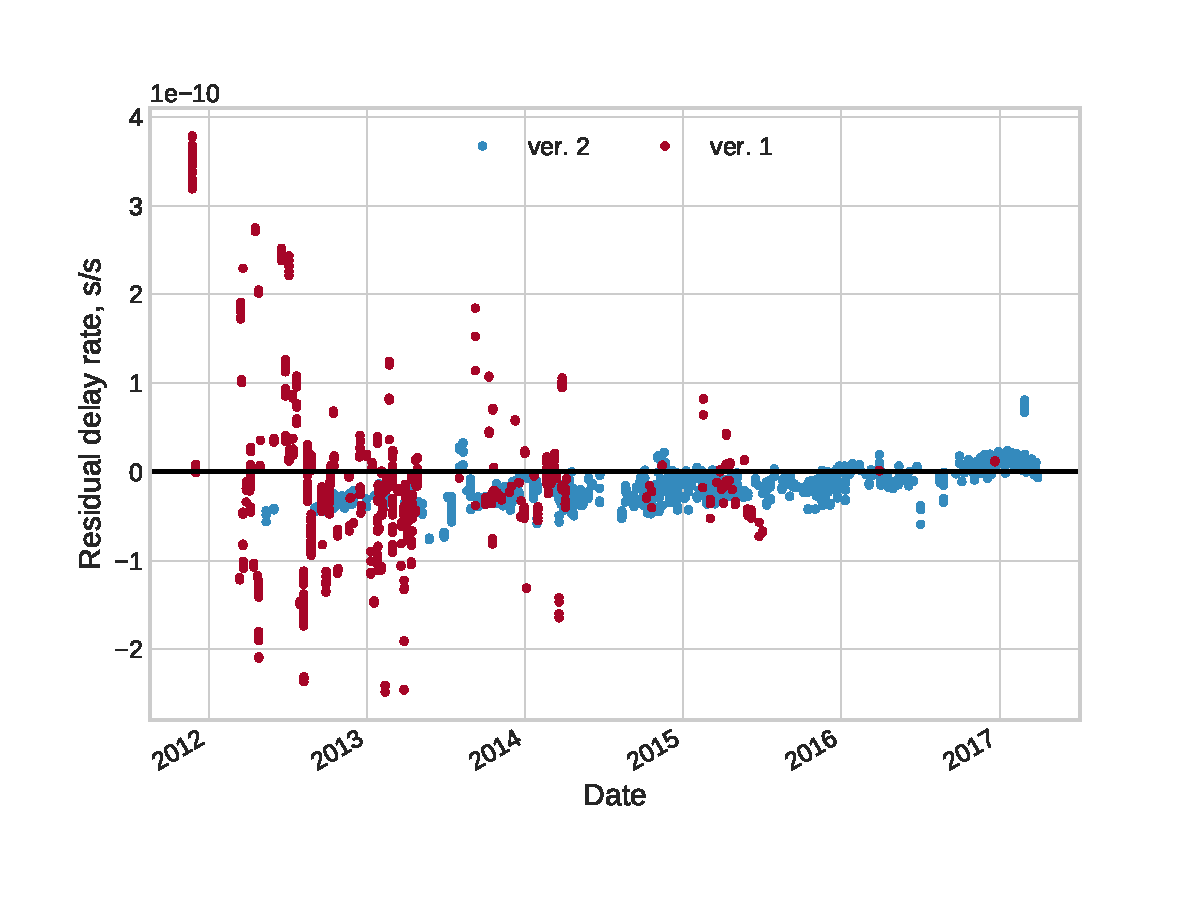
\includegraphics[width=0.7\textwidth]{raw_rrates_v1_v2.pdf}
 }
 \caption{Величины остаточной частоты задержки, полученные на корреляторе АКЦ с
использованием двух версий орбиты: универсальный алгоритм, версия 1 (красные точки); новый алгоритм,
версия 2 (синие точки). (Для интерпретации ссылок на цвет в этой легенде рисунка читатель обращается
к веб-версии этой статьи.)}
 \label{fig:rates_v1v2}
\end{figure}

На рис.~\ref{fig:rates_v1v2} показаны величины остаточной частоты задержки, полученные с помощью
коррелятора АКЦ в результате обработки наблюдений, выполненных миссией РадиоАстрон до начала 2017
года. Каждая точка данных на рис.~\ref{fig:rates_v1v2} соответствует значению остаточной частоты
задержки, определенной коррелятором. в результате корреляции двух сканов данных, то есть единиц
данных, обычно продолжительностью $\sim10$ минут, один из которых был записан космическим
радиотелескопом, а другой~"--- наземным радиотелескопом, который участвовал в эксперименте. Синие
точки обозначают остаточную частоту задержки, полученные с орбитами версии 2, т.е. те, которые
определены с помощью алгоритма, описанного в Разделе 4. Красные точки обозначают значения,
полученные на орбитах версии 1, т.е. определенные с помощью общего алгоритма OD и более простой
динамической модели космического аппарата. Более ранняя версия алгоритма использует простую модель
пушечного ядра для оценки SRP и, таким образом, игнорирует ее зависимость от ориентации. Кроме того,
изменения скорости из-за разгрузок не оцениваются в общем алгоритме, а устанавливаются на их
априорные значения. Для каждой точки на рис.~\ref{fig:rates_v1v2} предполагается, что КРТ является
первой антенной, а наземный радиотелескоп~"--- второй, то есть изображенные остаточные частоты
задержек являются относительными к космической антенне.

Все наблюдения, использованные для получения остаточных частот задержки на
рис.~\ref{fig:rates_v1v2}, проводились в так называемом однопутевом режиме, который
характеризуется следующими двумя условиями: (a) бортовое научное оборудование синхронизировано с
опорным сигнал бортового H-мазера; (b) несущая сигнала нисходящей линии связи, используемого для
передачи научных данных с космического аппарата на станцию слежения, также синхронизируется с
опорным сигналом H-мазера.

\begin{figure}[tbh]
 \centerfloat{
    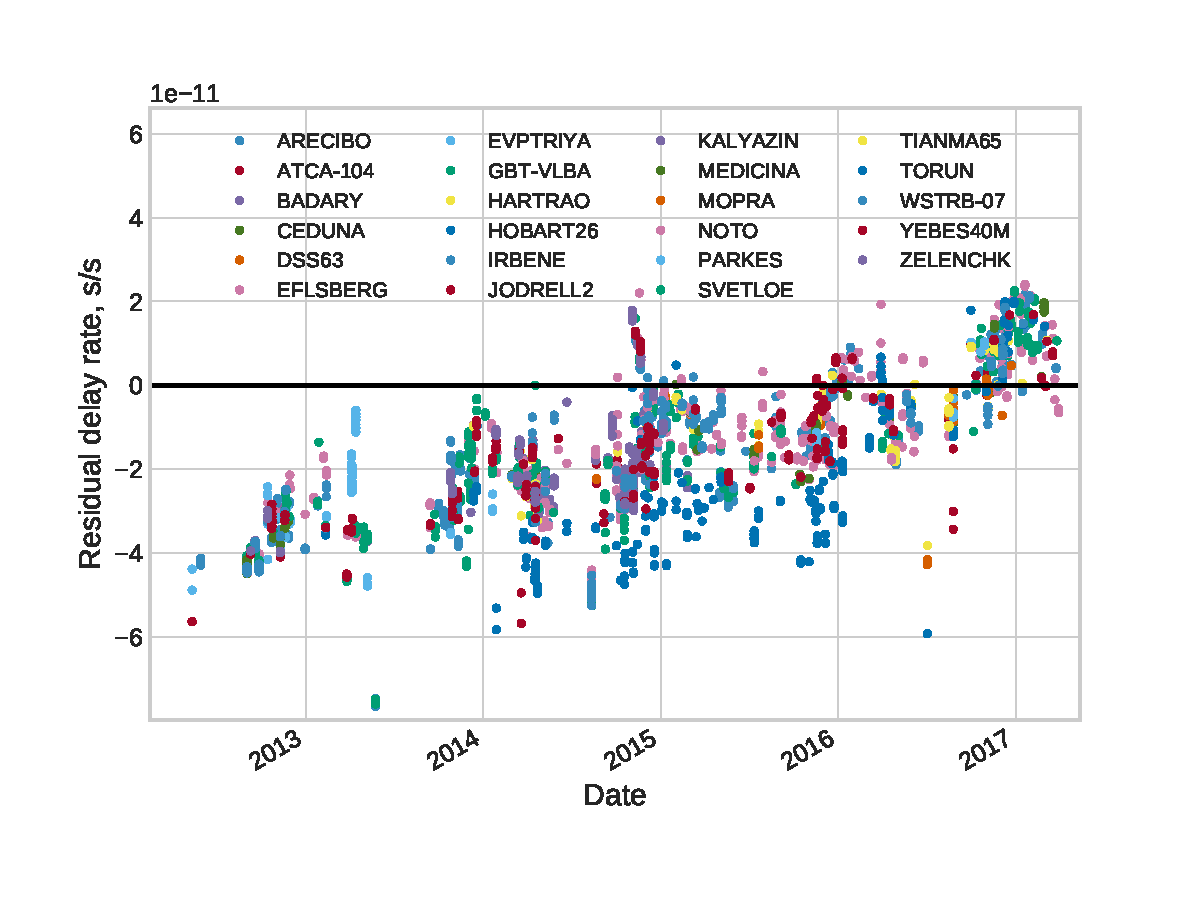
\includegraphics[width=0.7\textwidth]{raw_rrates.pdf}
 }
 \caption{Величины остаточной частоты задержки, полученные с использованием орбит версии 2. Цвет
указывает наземный радиотелескоп. (Для интерпретации ссылок на цвет в этой легенде
рисунка читатель обращается к веб-версии этой статьи.)}
 \label{fig:rrates}
\end{figure}

Из рисунка~\ref{fig:rates_v1v2} видно, что разброс остаточных частот задержки, полученных с
помощью версии 2 алгоритма OD, существенно меньше, чем у частот задержек, полученных с помощью
общего алгоритма. Среднеквадратическое значение остаточных частот задержек составляет
\num{2.463e-11} для версии 2 и \num{1.097e-10} для версии 1. Также ясно, что остаточные частоты
задержек, полученные на орбитах версии 2, смещены от нуля, а среднее значение равно
\num{1.663e-11}, а также показывают долгосрочный линейный тренд (рис.\ref{fig:rrates}). Последнее
явно указывает на систематический эффект, который нельзя отнести к ошибке OD, поскольку эти
остаточные значения были получены с использованием большого числа независимых решений и
еще большего числа наблюдений радиоисточников, рассеянных по всему небу и наблюдаемых на различных
проекциях баз.

\subsection{Выводы}

Мы изложили наш подход к определению орбиты космического аппарата РадиоАстрон. Этот метод включает
собственную модель давления солнечного излучения и алгоритм, позволяющий учесть накопленный момент
импульса маховиков для улучшения наших знаний о динамике центра масс космического аппарата.
Мы проверили эффективность этого метода определения орбиты, используя уникальные <<данные
слежения>>, доступные только для космического аппарата, участвующего в РСДБ наблюдениях, а именно
остаточные частоты задержек, которые в нашем случае были получены с помощью коррелятора АКЦ миссии
РадиоАстрон в результате обработки данных РСДБ-наблюдений небесных радиоисточников на КРТ совместно
с наземными радиотелескопами. Этот анализ позволил нам сделать вывод, что метод определения орбиты,
который мы разработали, обеспечивает до 11 раз более точные орбитальные решения с точки зрения
скорости и остаточных частот задержек по сравнению с обычным алгоритмом определения орбиты.
